\section{Psychological Exploitation of Social Engineering Attacks}
\label{intro} % Always give a unique label
% use \chaptermark{}
% to alter or adjust the chapter heading in the running head
\abstract{As cybersecurity tactics increasingly adapt to their environment, they introduce new complexities. In response, cybercriminals alter their attacks to be more elusive and discreet. Recent research underscores the prevalence of social engineering, in which cybercriminals manipulate the human element within an organization's security framework. Taking advantage of psychological traits, these attacks bypass technical defenses for nefarious purposes. Known as \textit{"human hacking"} or \textit{"hacking the human,"} social engineering represents a widespread tactic for targeting both individuals and organizations, often seen as an easier route compared to finding a technical vulnerability. These attacks are particularly difficult to counter because they lack consistent methodology, baselines, or patterns, making them incredibly potent and easy to disguise. Consequently, defenders must deepen their understanding of such attack techniques to effectively mitigate them. This chapter delves into the intricate methods employed in social engineering-based cyberattacks, examining how human vulnerabilities have been leveraged in recent breaches. Moreover, it explores current defensive strategies, including Machine Learning-based solutions, aimed at combating these attacks and protecting individuals.}

\begin{table}
    \justifying
\caption{Table 1: Summary of Topics Covered in Chapter}
\label{tab:placeholder}
    \begin{tabular}{cc}
         Section \& Summary\\
         Section 1: In this section, readers are introduced to the idea and workings of Social Engineering (SE) attacks. To highlight the importance of cyberattacks based on social engineering, some of the most recent and prominent attacks are presented.\\
         Section 2: This section covers the most common types of SE attacks and their prescribed methodologies.\\
         Section 3: In this section, methods of influence to exploit human vulnerabilities are discussed. This section also discusses the interrelated connections between SE attacks, methods of influence, human vulnerability exploitation, and how to counter SE attacks.\\
         Section 4: This section opens with the discussion of methods used to counter SE attacks providing readers with a deep understanding of the various countermeasures that can be used to combat these attacks, including some of the most prominent ML-based methods.\\
         Section 5: This final section raises concerns over recently proposed methods to counteract SE attacks emphasizing the need for a multidimensional approach to counter SE-based attacks and attack limitations.\\
    \end{tabular}
    
    
\end{table}


\subsection{Introduction}
"Our perimeter concerning human security is satisfactory. All employees participate in cybersecurity training periodically. How often, you ask? Well, annually, indeed, they undergo a one-hour session covering essential cyber hygiene practices. Additionally, the training addresses social engineering, specifically phishing and vishing threats. We are quite successful in these efforts."
While these dialogues typically occur within the protective confines of corporate conference rooms, there is a simultaneous exchange elsewhere—within clandestine online forums:
This is the detailed guide for executing my vishing strategy. The approach yields a success rate of 7 out of 10 instances. It is notably more effective when targeting small to medium-sized companies, as they typically lack comprehensive cybersecurity defenses. Prioritize ransomware attacks on organizations that possess cyber insurance; their lax attitude towards security results in faster payouts. Emphasize quality over quantity when identifying weak points. The sales team appears overwhelmed, making them an ideal initial target.
In a somewhat ironic twist, by the time security experts begin their work on Monday morning, cyber attackers and social engineers have already been busy. As the security teams commence their day, they engage in tasks such as reviewing the latest developments, addressing emails, and methodically progressing through their task lists, all aimed at fortifying their technical, physical, and human safeguards. On the other hand, adversaries are active every single day of the week, meticulously seeking out that singular vulnerability within an organization's security framework that could grant them access.
Cybercriminals consistently possess a significant asymmetrical edge, as they focus on uncovering just one exploitable weakness. Meanwhile, cybersecurity experts are tasked with safeguarding an organization across multiple layers of defense, advocating for increased budgets and the support of management and employees. They face complex choices and must prioritize specific security challenges above others to ensure comprehensive protection.
Currently, the digital realm is expanding at a remarkable pace. The internet is being increasingly adopted as an avenue for communication, commerce, education, and leisure. Yet, this significant transition has prompted critical online security and privacy issues for users. While stringent security protocols are in place, numerous cyberattacks occur due to exploiting application design flaws, fraudulent activities, or sophisticated technical tactics. Notably, scams have existed long before computers and the internet came about. In the realm of cybersecurity, scams or phishing are identified as Social Engineering (SE) attacks. These are attacks that target human weaknesses employing tactics such as deception, persuasion, manipulation, or influence.
Today's cyber security experts are consistently investing in bolstering technological defenses against cyber threats. However, as reflected in numerous threat analyses published in recent years, modern cyber criminals increasingly target people as it is a more straightforward approach than attacking technology. Despite continuous advancements in security technology that improve system resilience and complexity, human nature has remained constant for centuries, making it predictable and exploitable. This method is both cost-effective and low-risk, yielding significant benefits for cyber criminals. Rather than merely applying brute force techniques on an organization's passwords, attackers can exploit psychological tactics to manipulate an unsuspecting employee into divulging passwords and other sensitive credentials.
It is logical to assert that employees with access to an organization's vital resources become prime targets for social engineering schemes. The aim of such attacks is to manipulate employees into granting access to systems, assets, or confidential data. Those with access to technological and organizational resources bear the responsibility for safeguarding them. However, are these employees adequately equipped and qualified for this duty? Are they sufficiently aware and skilled to fulfill these expectations and defend their assets against threats posed by malicious actors and social engineering tactics?
A major challenge in today's cyber security efforts is the lack of \textit{effective }information security awareness and training. Many organizations and companies of the public and the private sector continue to believe that cyber security is only a technical, not a strategic and behavioral discipline. They believe that cyber security involves only the protection of systems from threats like unauthorized access, not the awareness and training of persons that have authorized access to systems, information and organizational assets. Therefore, they invest significantly less in any processes or measures that have to do with the human perimeter of their organization.

This becomes a susceptibility within the organization that can be capitalized on. It represents an oversight that adversaries are all too eager to take advantage of.
\textbf{Engineers of Human Behavior}

The core principle of Social Engineering revolves around harnessing human psychology. Opponents strategically apply psychological tactics, using deceit and manipulation to target innate decision-making processes that influence actions and incentives. Human vulnerabilities exhibit predictable stimulus-response patterns, making the exploitation of these weaknesses reliably effective; however, before examining the psychological manipulation aspect, it is crucial to first explore the expertise and approach employed by social engineers.
Social engineers excel at studying and understanding human behavior. They often possess innate social talents, show charm, or have a keen interest in understanding human nature and honing the skill of reading others. By practicing, they master the recognition of emotions and thoughts conveyed through nonverbal cues, including body language and vocal intonation. This ability is crucial, as it enables them to steer conversations and influence their targets by attentively observing reactions and adapting their own strategies accordingly.
When interacting with individuals, do they appear cautious or suspicious? If so, they retreat and work to build trust. Should this effort fail, they realize that they must abandon this target, as persisting might be perilous. Conversely, if they detect that sufficient trust and possibly likability have been ingrained, they proceed to make bolder requests that promise higher rewards. It resembles executing a meticulously developed algorithm on human actions. This implies that social engineers dynamically tailor their deceit strategy based on their targets' responses, continuously refining their approach in real-time. By modifying their own actions, they effectively "engineer" and steer the conduct of those they are engaging with.
However, there is more to consider. Skilled social engineers conduct thorough research on their targets' backgrounds before engaging them. This process typically involves aggregating snippets of data from sources such as social media, blog posts, or simply by distant observation. They meticulously analyze their targets' professional schedules, behaviors, dialogues, and any other details that provide insight into their daily routines, mental processes, and behavioral trends. Armed with this intelligence, they strategize their approach to align seamlessly with their targets' profiles. The objective is to quickly capture the target and establish immediate trust in their initial interaction. This early foundation of trust becomes crucial in facilitating the subsequent stages of the attack.
The ultimate aim of social engineers is to persuade their targets to willingly disclose confidential information or grant access to corporate systems and resources. Typically, victims assist these covert social engineers, either out of a perceived benefit or simply due to their enjoyment of the interaction, without realizing that their actions might jeopardize their organizations.\begin{figure}
    \justifying
    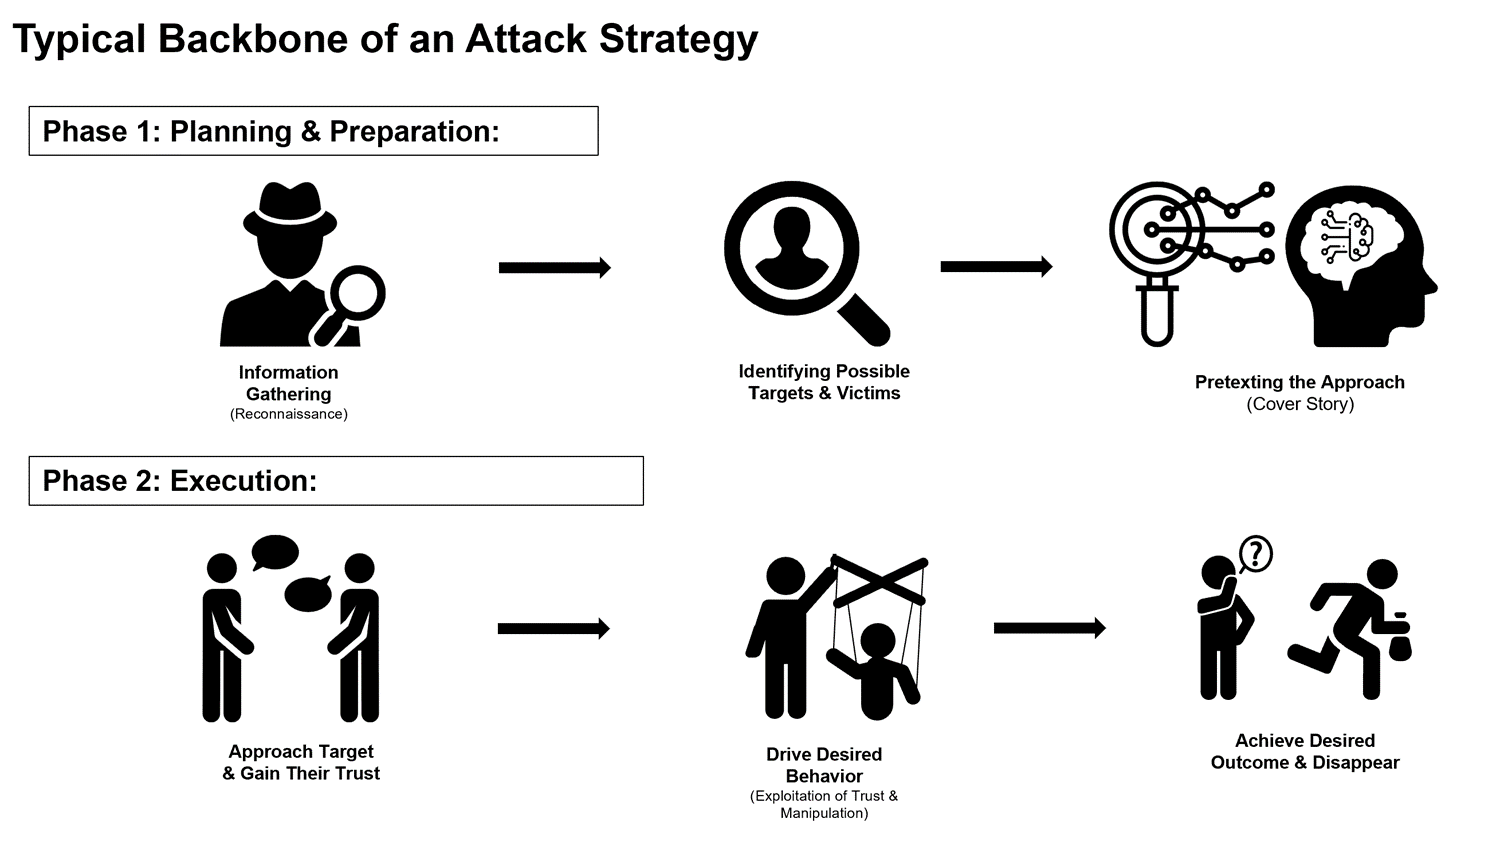
\includegraphics[width=0.75\linewidth]{socengattstr.png}
    \caption{Enter Caption}
    \label{fig:placeholder}
\end{figure}
 
Social engineering is an art and science that combines both technical and behavioral skills, with the emphasis on behavioral rather than technical. The remainder of this section will discuss some of the very common social engineering approaches along with the analysis of the psychological exploitation that comes into play for a successful attack; however, while there are some common approaches or scenarios, the potential amount of social engineering methodologies and scenarios can be endless and ultimately depend on the attacker's creative imagination and influential capability.

\textbf{Programming The Trust Algorithm}

No social engineering attacks would be possible if the attackers were not able to first build trust with their targets. Whether the attack vector is emails, the phone, or a personal interaction, victims must first believe the cover story delivered by the attackers. Only then they will take the next steps that the social engineers indicate that eventually lead to an effective compromise.

But how can someone program the trust process of another individual? Is it even possible to engineer a trust relationship? The answer is yes. In fact, the field of psychology teaches us that there are multiple ways to establish trust with someone. Unfortunately, the rules of trust are the same in both honest and deceptive relationships. This is also the reason why it is often hard to differentiate one from the other when encountering an individual or a communication request (e.g. email or phone call).

Let us start from scratch. All humans naturally pay attention to a few key elements when encountering someone for the first time. These are some of the mental questions that go through our heads, often without even realizing that:

- “I like him/her” (or the opposite)
- 'Who is this person?'
- 'Why is this person reaching out to me?'
- Does he / she have authority over me?

Social engineers know these mental questions, and the fact that we go through this mental checklist within milliseconds of a first interaction. These are the so-called “cognitive filters” we all have in order to evaluate another individual. Social engineers make sure they have good answers to these mental questions, in order to immediately hack-through the walls of our initial suspicion and gain a quick trust advantage. They do that, by heavily relying on psychological principles that all of us are used to operate by.

Therefore, social engineers often tend to use cover stories that tend to include:

\textbf{Persons or organizations with authority}

People tend to assign immediate trust to authoritative figures and not doubt their intention. Social engineers will impersonate company executives, lawyers or technicians. The attackers have already investigated which authoritative figures are suitable for each of their victims.

\textbf{Social Proof}

People are more willing to do something or trust a situation or interpersonal dynamic when they observe other people doing it first. They also put a lot of weight into other people’s endorsements. Psychological studies repeatedly show that we often evaluate a situation based on what other people think of it. Social engineers exploit this principle by name-dropping. They might contact a target by first mentioning that someone else (often with authority over the target) recommended that they must communicate with the target. Or they initiate contact by saying that they are currently replacing another specific person from a partner company the target used to communicate with. The social engineers then can proceed by engaging the targets in conversations with the goal of gathering information, or by sending malicious emails and cashing on the trust they have established with the targets through social proof.

\textbf{Consistency}

This is a highly valued trait in today’s society. People associate consistent behaviours with people that are reliable, intelligent, trustworthy, and other highly praised traits. Due to this social norm, people tend to care a lot about appearing consistent. Once someone has made a choice or has taken a stand, they go through great personal and interpersonal pressure to defend that stance. Social engineers often use this principle to gather sensitive information. Once they have made their targets answer small or innocent requests, they request more valuable information. Most often their targets, since they have already gotten in the habit of answering, feel an inner pressure to keep replying to the questions and self-justifying the reasons they do so, even when they start becoming uncomfortable or suspicious. As the conversation progresses, it also becomes harder to turn down the persons they are interacting with.

\textbf{Liking}

People like people who are similar to them, or who show admiration to them. When people are similar to us, we tend to perceive them as belonging to “our tribe”. Psychological studies have shown that when people appear to be or think like we do, we automatically assign some other psychological characteristics to them. Specifically, we automatically assume that they also share similar backgrounds, way of thinking, and more. Our brains, being highly automated, immediately translate this into trustworthiness. Social engineers invest heavily in building rapport with their targets and work hard to increase their likeability and level of trust.

People prefer to open up and respond positively to requests from people they like. The targets of this approach tend to drop their mental guards rather quickly. The result? They are much more likely to answer questions and provide information, as well as bypass security policies by opening malicious email attachments, or even open physical security doors to the social engineer that is of course, impersonating someone else.

\textbf{Scarcity}

The thought of loosing an attractive opportunity or missing on a “limited availability” offer tends to hold a lot of weight in the human decision making process. Items that are limited or scarce, are frequently perceived as more valuable and more attractive. This creates desire. But it also creates a sense of urgency. Combined, they make people more than willing to take more than a few shortcuts on the critical thinking processes. In marketing, this principle is at full-force when marketers make statements like “this item is selling fast- only 5 left in stock!” or “this is a limited edition item”. In social engineering, we can see this approach in the phishing email scenarios where the targets are promised to “receive 1 of the 15 iPads/iPhones/expensive gadgets available by filling in a survey”, or “rush to claim their reward” (by clicking on a malicious link). We can also see this approach when a social engineer places a vishing call, impersonating someone with authority, and claims that they only have 15 minutes to resolve an issue. This tactic connects with the principle of “time pressure” (below).

\textbf{Urgency/ Time pressure}

Time pressure is a motivating factor connected to the one of scarcity, not in terms of making an action desirable, but in terms of giving someone a very short amount of time to fulfil a request. The time pressure is often big enough to make one skip essential critical thinking and analytical processes while acting on a request. Social engineers benefit a lot by making their targets skip any real thinking processes. Ideally, they want their targets to operate without thinking at all. Therefore, plenty of the social engineering scenarios (pretexts) involve the factor of time pressure or other tactics that block our critical thinking. These attacks may come in the form of spear phishing emails impersonating executives claiming that they want an immediate transfer of funds to a specific account, while adding that the matter is time-sensitive. Or it may come in the form of a vishing call from social engineers impersonating technicians, stating that they need to run a few remote updates within the next hour and therefore would need the login credentials of employees, or other sensitive information.

These are only some of the psychological principles that social engineers repeatedly try to exploit. They often combine them, to increase their level of influence.

\textbf{Incorporating Psychological Pressure into Attack Scenarios}

Attackers keep using old and tried cover stories that have proven to be consistently successful, because these stories involve the exploitation of the psychological principles mentioned above. One common attack scenario is the vishing (phone-based) attack, where the attackers call employees and pretend to be IT support staffers. Then they proceed to explain their cover story: For example, they may say that they are running some critical system upgrades and that they need an employee’s username and password in order to proceed. Or they may say that they have developed a new online communication platform for employees and ask them to register for it through a phishing email that they consecutively send, containing a malicious link. They utilize the principle of authority over the target’s technical infrastructure and may include a component of urgency by notifying their targets that their update needs to happen immediately. Although this social engineering scenario has been known for years, attackers keep using it and unfortunately, it still works.

Users can recognize an attack from certain red flags. For example, many social engineering pretexts use the combination of fear and time pressure to push an employee towards immediate action - this is an immediate red flag. Also, no matter what the cover story is, most attacks boil down to specific requests that should make an employee suspicious. For example, requests for sensitive information, or requests to click a link. Employees need to learn how to recognize the red flags, how to respond to them, and how to verify the contact person in a business-appropriate manner. This happens through training.

\textbf{Human Zero-day Exploits}

Although many social engineering techniques or scenarios are known, there are many that are not. Some of them are often associated with higher exploitation potential for high value targets. Social engineers thoroughly investigate their targets and can adopt an approach that is tailored to each specific target, in ways that it is difficult to detect the attack. The high value targets are often members of the C-Suite, executives, or people with important access privileges.

When determined social engineers target more difficult, yet rewarding targets, they put in the time and effort to analyse these specific targets as well as possible. They may seek to find their routines, interests, habits, physical locations, etc. But what they are most interested in, are their psychological characteristics, vulnerabilities and overall psychological profiles. Threat actors have a deep knowledge of psychology, have better resources and capabilities, and often belong to an organized group. They utilize psychological profiles they craft by seeking to identify and exploit personal characteristics of the targets they seek to victimize.

They will find a way to physically or virtually approach their victims with tempting personas and build a relationship with them. Alternatively, they may choose to blackmail their victims, or recruiting them. These types of attacks are based on personal human vulnerabilities of the targets that even the victims themselves might not be aware of, and even more certainly so, the security teams that work in their organization. These are the Human Zero-day exploits. For persons that have priviledges and access rights critical for an organization, specialized security experts must come in to conduct a \textit{personal vulnerability assessment,} and proceed with personalized training based on the assessment.

\textbf{Epilogue}

We cannot fully protect employees against social engineering attacks. What we can do, is teach them how to protect themselves and their organizations. The most exploitable factor in social engineering is ignorance. A person that does not know the tactics and methods used from social engineers, is defenceless against them.

Social engineers target our employees directly and seek to have an encounter with them. Sooner or later some of our employees will get targeted again by attackers. When this occurs, they will have to:

a) Identify that this is an attempt for a social engineering attack,

b) Respond to the attack by gracefully disengaging,

c) Report it to their organization (given that a reporting mechanism is in place).

They must understand that security is a shared responsibility, and that they play a significant role in it. At the same time, security professionals must understand that this is a growing threat and one that will keep being exploited, unless we build up more knowledge and skills within our organization to combat these attacks. This effort must be supported by a good cybersecurity culture. While attackers develop their skillset and invest time, resources and strategic thinking, it is not enough for us to simply inform employees about the threats. We must build their skillset in recognizing and defending against them, which can only be done with targeted employee trainings. Ideally in person, and more than once per year for 60 minutes.

The mentioned vulnerabilities are exploited to acquire confidential information, unauthorized access, knowledge of cybersecurity measures, etc. The main concern for security experts in countering SE-based attacks is the absence of a pattern or methodology. In some cases, even the target is unaware that they are being manipulated or influenced by the perpetrator. Due to such hazy characteristics of SE-based attacks, existing countermeasures struggle to stop such attacks. Recently, there were several large-scale security breaches, compromising the vulnerable human factor. Despite the advancements in technology, humans play an integral part in functional organization. This human element in the organizational security chain is inevitably targeted and exploited by hackers. Figure 1 shows some of the most common tools and a basic flow of cyberattacks based on SE.
\begin{figure}
    \justifying
    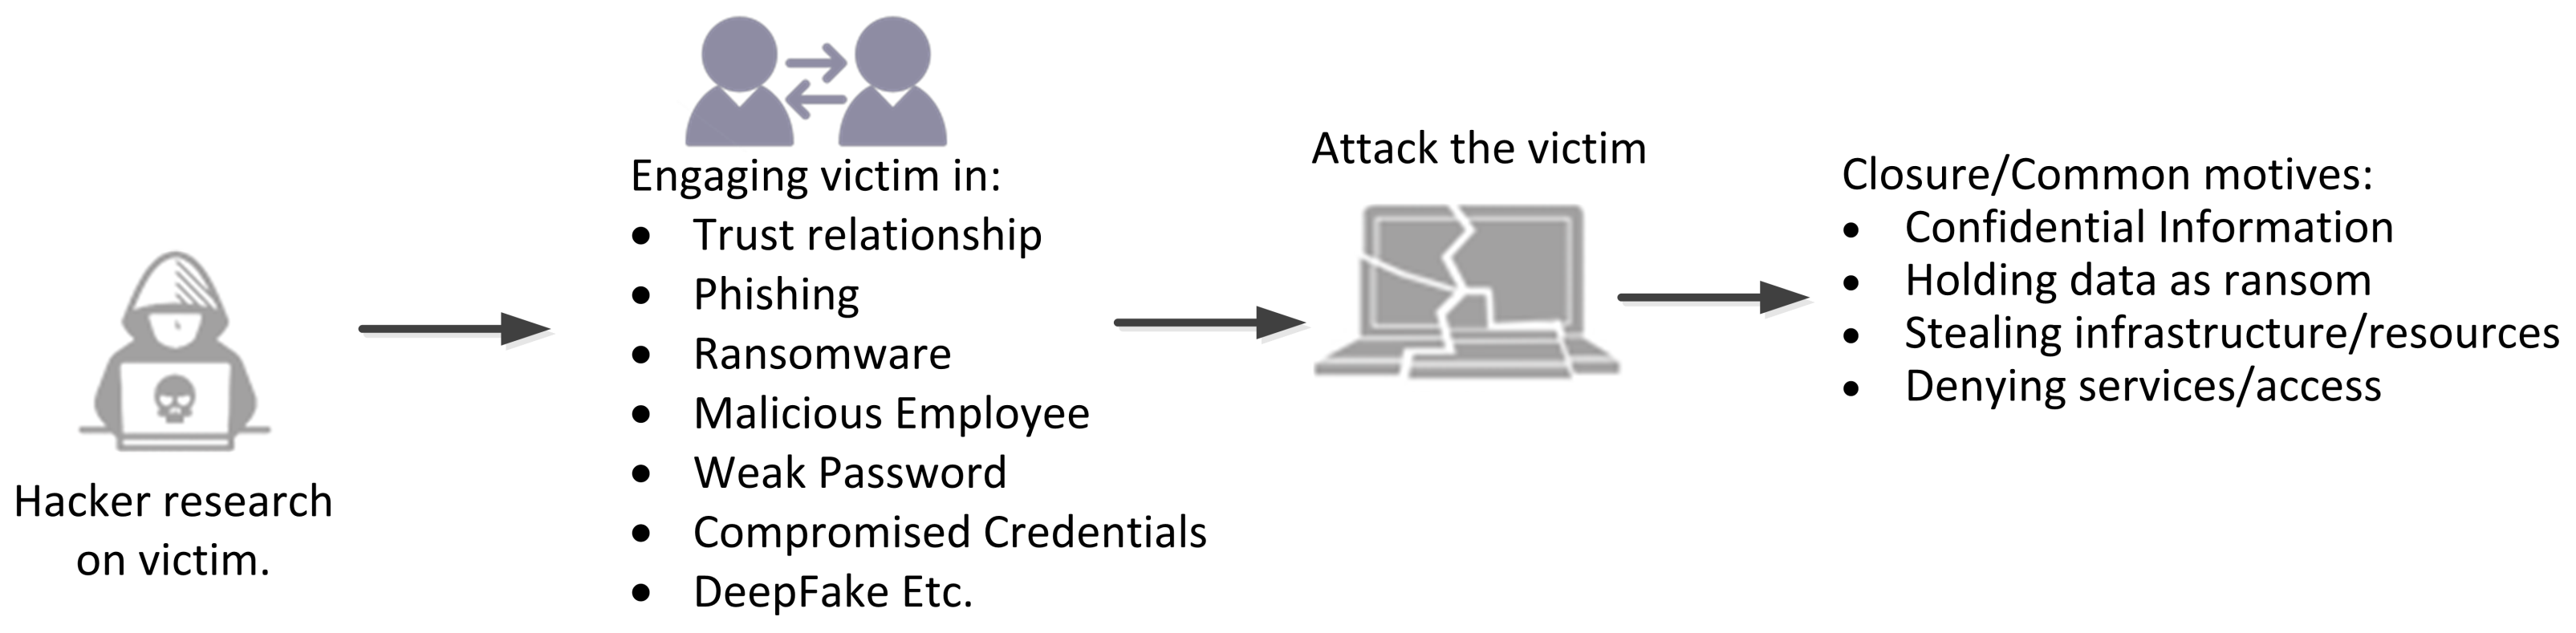
\includegraphics[width=0.75\linewidth]{socengflow.png}
    \caption{Enter Caption}
    \label{fig:placeholder}
\end{figure}
 In the last two years, the most prominent mediums used to conduct SE attacks were social media and smishing attacks. The majority of cyberattacks based on SE rely on actual interactions between the attacker and the victim. In some cases, SE attacks can involve a simple phone call, with an individual impersonating an employee to garner information, such as a password or a PIN code. In 2020, Americans lost approximately USD 29.8 billion in phone scams [\href{https://www.mdpi.com/2076-3417/12/12/6042\#B10-applsci-12-06042}{\textbf{10}}]. \href{https://www.mdpi.com/2076-3417/12/12/6042\#table_body_display_applsci-12-06042-t001}{\textbf{Table 1}} provides a broad overview of attacks based on SE methods. The attacks highlighted in \href{https://www.mdpi.com/2076-3417/12/12/6042\#table_body_display_applsci-12-06042-t001}{\textbf{Table 1}} are some of the most prominent breaches in the last few years. These breaches occurred due to a combination of human errors and SE attacks. Based on \href{https://www.mdpi.com/2076-3417/12/12/6042\#table_body_display_applsci-12-06042-t001}{\textbf{Table 1}}, it can be seen that human error can also play a key role in conducting SE attacks. To conduct SE attacks, hackers can even influence a victim into making an error. Common methods used to influence targets are discussed later in the chapter. Other than the financial costs, data breaches can also lead to the loss of customers due to security concerns. These attacks are highly impactful and easy to conduct. Based on the studies conducted for this work, as well as our understanding, the countermeasures for SE-based attacks lack the understanding of human behavior. Few of the published works highlight the interconnection between human vulnerabilities and SE attacks. This study further enhances the existing knowledge of human behavioral vulnerabilities and how they are exploited by hackers. After highlighting the importance and impact of cyberattacks based on SE, the rest of the chapter is organized as follows. \href{https://www.mdpi.com/2076-3417/12/12/6042\#sec2-applsci-12-06042}{\textbf{Section 2}} provides a brief overview of well-known cyberattacks based on SE and how they are conducted. \href{https://www.mdpi.com/2076-3417/12/12/6042\#sec3-applsci-12-06042}{\textbf{Section 3}} provides a perspective on common human emotions or errors that can be exploited to conduct SE attacks. The section also presents the current standings and concerns of machine learning (ML) and existing countermeasures against SE-based cyberattacks. \href{https://www.mdpi.com/2076-3417/12/12/6042\#sec4-applsci-12-06042}{\textbf{Section 4}} highlights the concerns of existing solutions, including a summary of the topics discussed in this chapter. \href{https://www.mdpi.com/2076-3417/12/12/6042\#sec5-applsci-12-06042}{\textbf{Section 5}} concludes the chapter.


 \textbf{Table 1.} Some of the most prominent social engineering-based cyberattacks.


\subsection{\textbf{2. Social Engineering Attacks}}

Social engineering can be defined as a process used to exploit human psychology, rather than a sophisticated hacking method [\href{https://www.mdpi.com/2076-3417/12/12/6042\#B18-applsci-12-06042}{\textbf{18}}]. With growing reliance on technology, SE is becoming a key tool for cyberattacks. Conversely, due to the increasing number of cyberattacks, the technical methods used to counter cyberattacks are also improving [\href{https://www.mdpi.com/2076-3417/12/12/6042\#B19-applsci-12-06042}{\textbf{19}}]. These continuous improvements of security methods are making technical attacks difficult to execute. On the other hand, SE is proving to be a highly successful approach used to conduct cyberattacks. Cyberattacks based on SE can facilitate attackers in several ways, i.e., infiltrating organizational networks, bypassing firewalls, infecting systems with malware, opening back-doors in the organization network, etc. Cyberattacks that use SE can exploit or influence human behavior in many ways. For instance, human error can be used to initiate an attack. Attackers can enforce an individual to err by influencing the decision-making process. Details on how decision-making is influenced are discussed later in the chapter. Similarly, several other human behaviors can be exploited to conduct cyberattacks based on SE [\href{https://www.mdpi.com/2076-3417/12/12/6042\#B20-applsci-12-06042}{\textbf{20}}]. In this section, some of the most common cyberattacks based on SE are discussed.

\paragraph{\textit{2.1. Phishing Attack}}

Phishing attacks are among the most successful attack methods in SE-based attacks. Each day, millions of scam emails are sent by hackers, some are detected and blocked by different technical solutions [\href{https://www.mdpi.com/2076-3417/12/12/6042\#B21-applsci-12-06042}{\textbf{21}}]. However, some scam emails do manage to evade these systems. Phishing attacks typically start with a scam email that lures a victim into a trap. For instance, a phishing email may appear to come from an authentic source.The method of luring a victim can vary depending on who the victim is, i.e., the email may ask the victim to click the link for your travel expense receipt, click the link to win a prize, etc. Falling victim to such phishing emails is based on human behavior attributes [\href{https://www.mdpi.com/2076-3417/12/12/6042\#B22-applsci-12-06042}{\textbf{22}},\href{https://www.mdpi.com/2076-3417/12/12/6042\#B23-applsci-12-06042}{\textbf{23}}]. The process of a common phishing attack can be seen in \href{https://www.mdpi.com/2076-3417/12/12/6042\#fig_body_display_applsci-12-06042-f002}{\textbf{Figure 2}}. A phishing attack can be conducted in several different ways. Two of the most common methods can be seen in \href{https://www.mdpi.com/2076-3417/12/12/6042\#fig_body_display_applsci-12-06042-f002}{\textbf{Figure 2}}. As these attacks evolve, the goal of any type of phishing attack is to steal personal credentials or information. Some phishing attack types can be seen in \href{https://www.mdpi.com/2076-3417/12/12/6042\#table_body_display_applsci-12-06042-t002}{\textbf{Table 2}} [\href{https://www.mdpi.com/2076-3417/12/12/6042\#B24-applsci-12-06042}{\textbf{24}},\href{https://www.mdpi.com/2076-3417/12/12/6042\#B25-applsci-12-06042}{\textbf{25}}].
\begin{figure}
    \justifying
    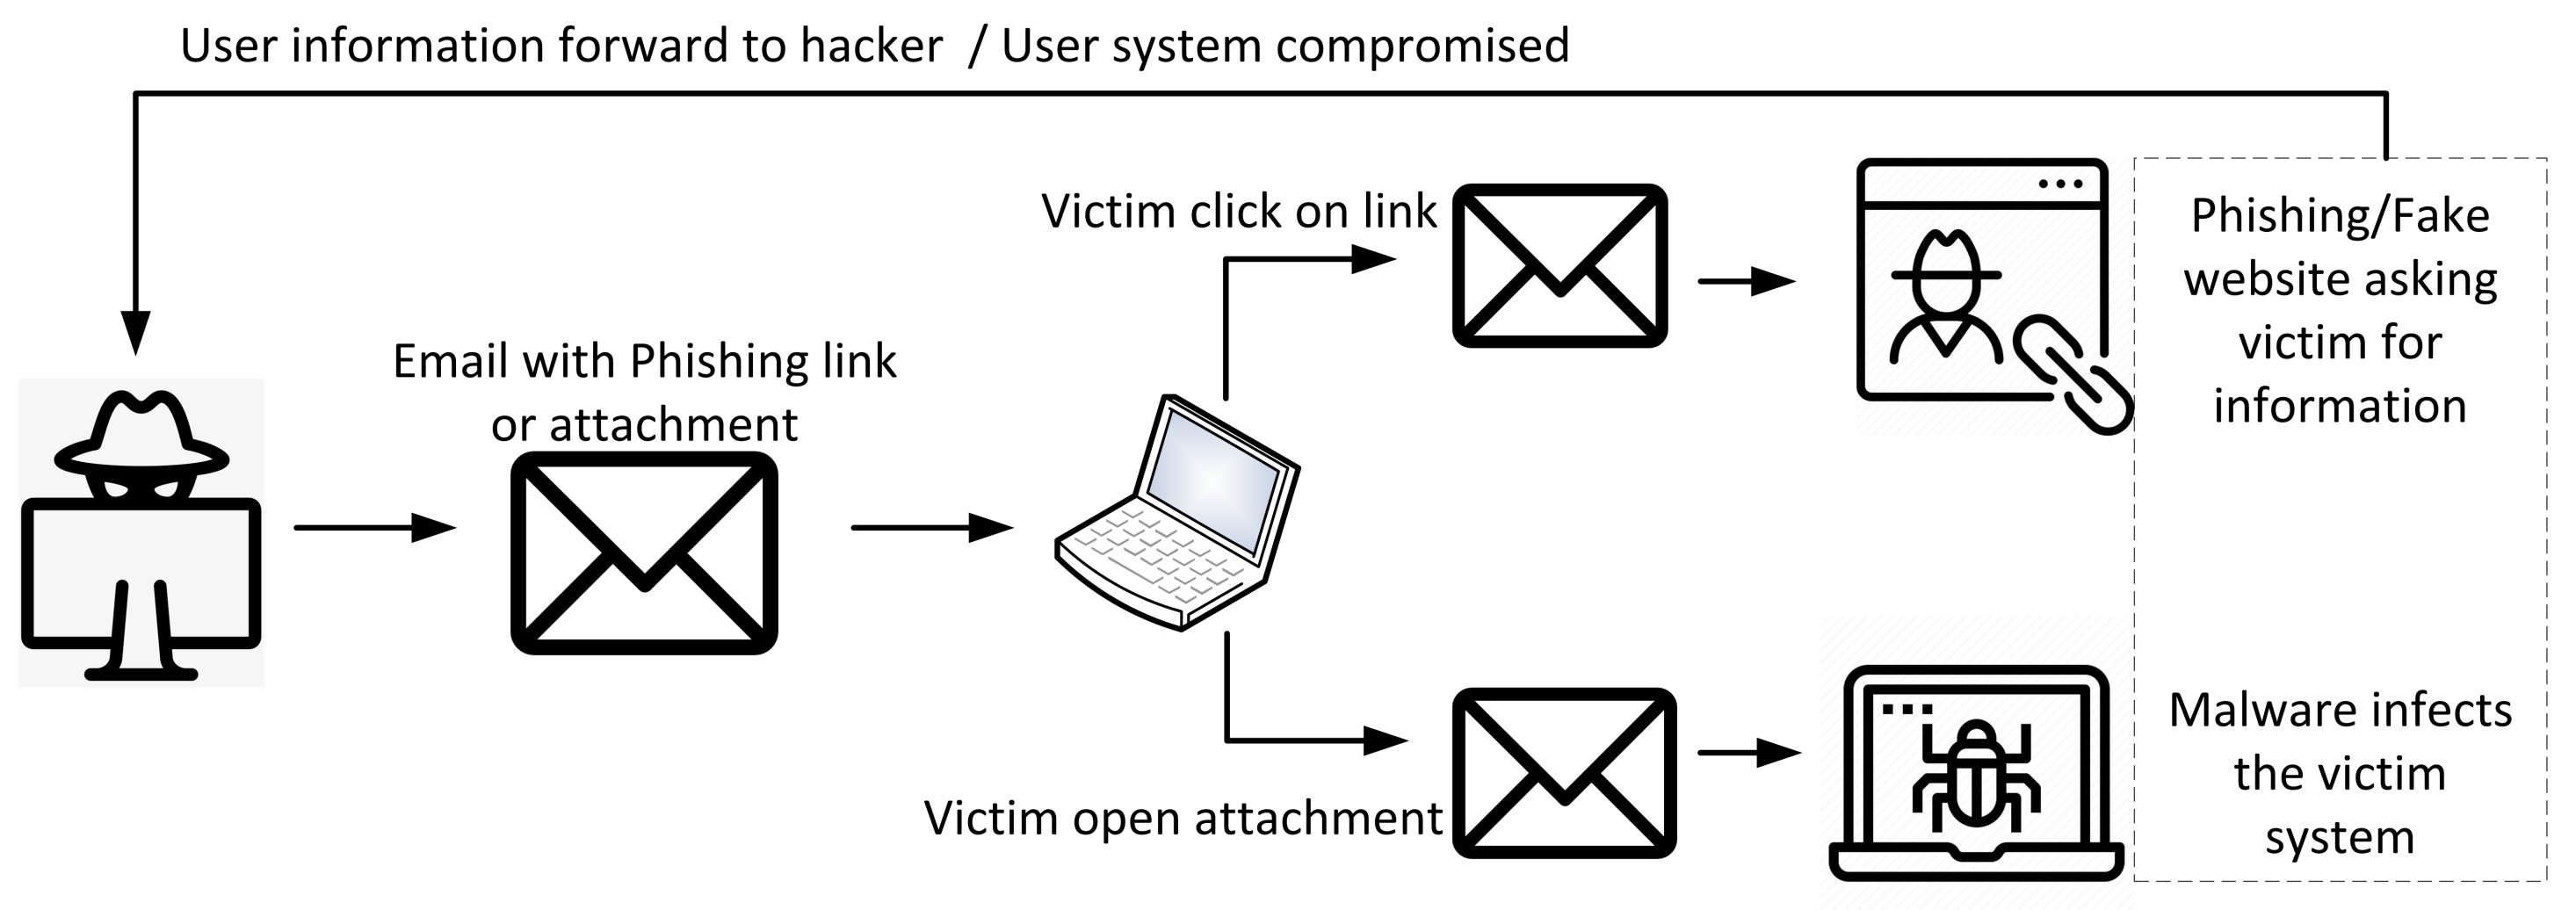
\includegraphics[width=0.75\linewidth]{phishingflow.png}
%\caption\textbf{Figure 2.} The common flow of phishing attacks.
    \label{fig:placeholder}
\end{figure}
\textbf{Table 2.} Common types of phishing attacks.
 
\paragraph{\textit{2.2. Dumpster Diving}}

The dumpster diving attack is a low-tech method used to obtain information on the target [\href{https://www.mdpi.com/2076-3417/12/12/6042\#B26-applsci-12-06042}{\textbf{26}}]. The process involves going through trash and looking for torn documents, receipts, and other forms of chapter that could contain information on the target. An individual may throw away a piece of chapter that may contain information about a password, pay slip, bill, credit card information, or something containing critical information. Such information can help hackers with several methods to conduct a SE attack on an individual. Dumpster diving is also among the most common methods of identity theft [\href{https://www.mdpi.com/2076-3417/12/12/6042\#B27-applsci-12-06042}{\textbf{27}}]. \href{https://www.mdpi.com/2076-3417/12/12/6042\#fig_body_display_applsci-12-06042-f003}{\textbf{Figure 3}} elaborates on some of the content that can be found in an organization’s dumpster. As seen in \href{https://www.mdpi.com/2076-3417/12/12/6042\#fig_body_display_applsci-12-06042-f003}{\textbf{Figure 3}}, the dumpster could contain any of the mentioned information. Normally these documents or chapters are torn and thrown into the trash. A malicious actor can go through the dumpster and retrieve information to assist in conducting a SE-based attack. 
\begin{figure}
    \justifying
    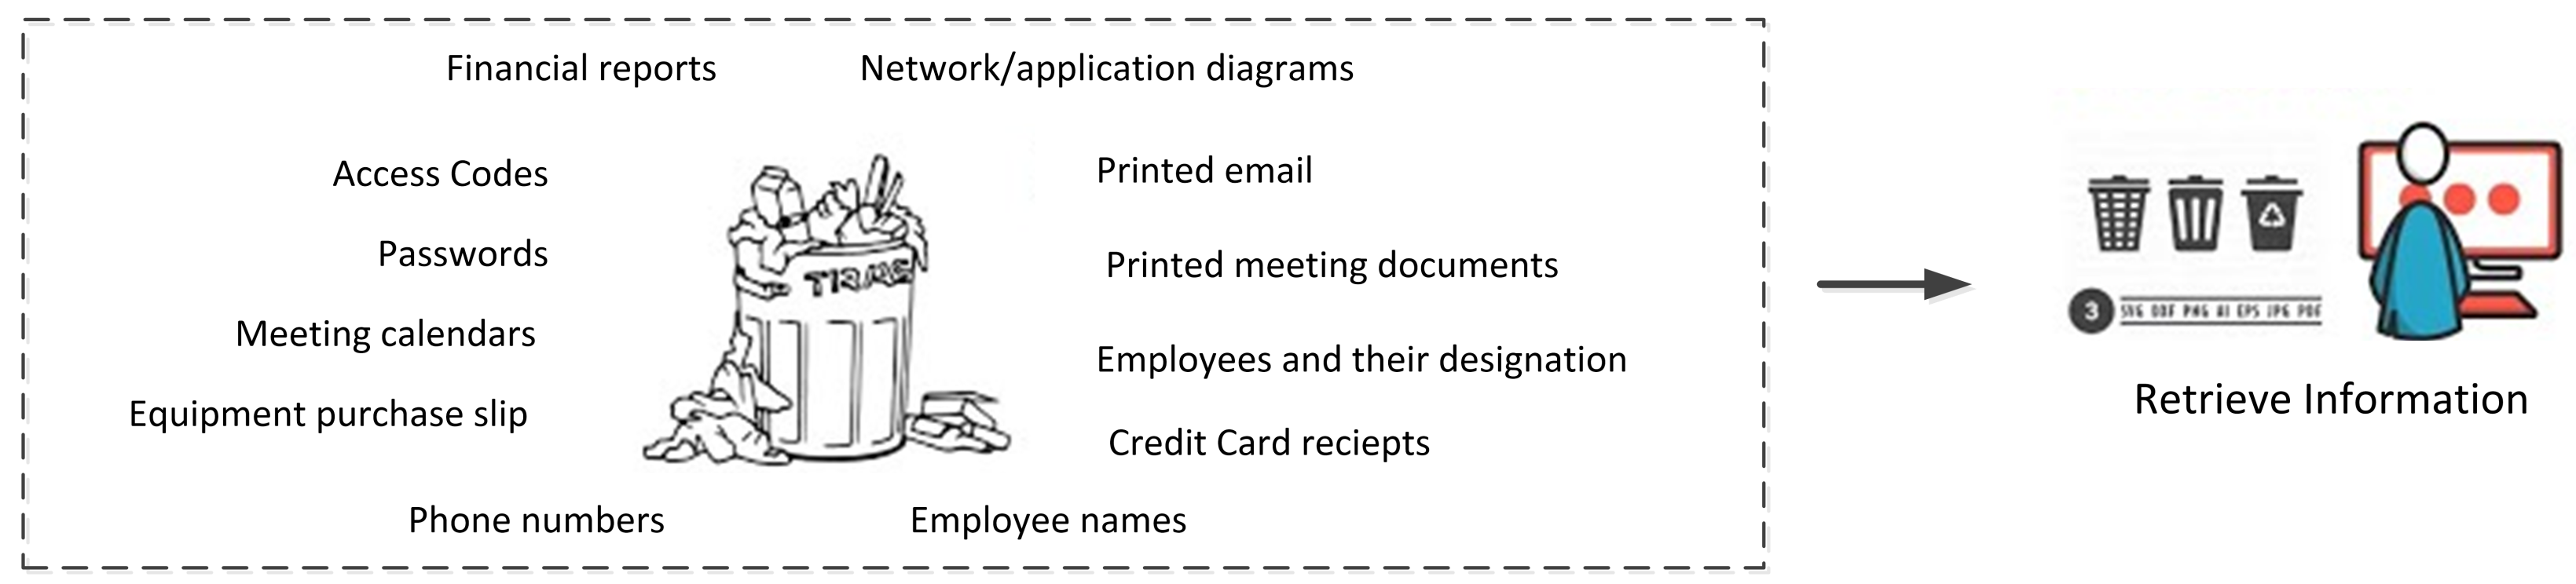
\includegraphics[width=0.75\linewidth]{dumpsterdive.png}
    \caption{\textbf{Figure 3.} Content that can be found via dumpster-diving in an organization’s trash.}
    \label{fig:placeholder}
\end{figure}

\paragraph{\textit{2.3. Scareware}}

Scareware can be defined as a type of SE attack that is based on human emotions, i.e., anxiety, shock, manipulation, etc. [\href{https://www.mdpi.com/2076-3417/12/12/6042\#B28-applsci-12-06042}{\textbf{28}}]. The attack uses human emotions to manipulate the user into installing malicious software. The steps involved in a scareware attack can be seen in \href{https://www.mdpi.com/2076-3417/12/12/6042\#fig_body_display_applsci-12-06042-f004}{\textbf{Figure 4}} [\href{https://www.mdpi.com/2076-3417/12/12/6042\#B29-applsci-12-06042}{\textbf{29}}]. It can be seen (in \href{https://www.mdpi.com/2076-3417/12/12/6042\#fig_body_display_applsci-12-06042-f004}{\textbf{Figure 4}}) that hackers use pop-up-based alerts on different sites to engage the target. Once the target clicks the pop-up, he/she is targeted using misinformation. The misinformation is intended to influence the target to perform an act out of panic. The intended act may ask the target for sensitive information or to buy a product to solve the fake issue. In a scareware attack, the hacker only needs to persuade the victim to click on a link. For this persuasion, the attacker can use numerous techniques to influence the victim into installing the scareware malware. The graphical interface of scareware is in many ways an integral part of deceiving victims. The visual representation of the scareware (e.g., a pop-up or a scan report) meritoriously presents a credible and trustworthy application. Most forms of scareware malware adopt color schemes, font styles, and logos that are similar to known brands of antivirus or software products, e.g., Microsoft, Norton antivirus, etc. [\href{https://www.mdpi.com/2076-3417/12/12/6042\#B29-applsci-12-06042}{\textbf{29}}].


% \begin{figure}
     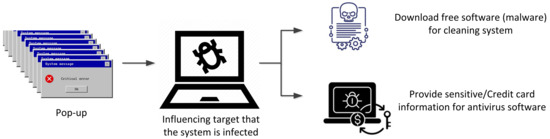
\includegraphics[width=0.75\linewidth]{scareware.png}
  %   \caption\textbf{Figure 4.} Steps of a scareware attack.
     \label{fig:placeholder}
 %\end{figure}
 
\paragraph{\textit{2.4. Water Hole}}

A water hole attack or water holing is a SE attack inspired by the hunting method of predators in the jungle. In the real world, the predators in the jungle wait near a water hole to attack their prey [\href{https://www.mdpi.com/2076-3417/12/12/6042\#B30-applsci-12-06042}{\textbf{30}}]. \href{https://www.mdpi.com/2076-3417/12/12/6042\#fig_body_display_applsci-12-06042-f005}{\textbf{Figure 5}} provides an overview of how a water hole attack is commonly conducted [\href{https://www.mdpi.com/2076-3417/12/12/6042\#B31-applsci-12-06042}{\textbf{31}}]. In step one, the attacker identifies the organization to target, then uses surveys and other means to identify the browsing habits of the employees. Based on this information, the hackers identify the frequently visited website by the employees. In step two, the attacker compromises the legitimate website. Compromising a secure site could be near impossible, so hackers must identify the website that can be compromised (one that is frequently visited by the employees). In step three, the hackers direct the employee from the original website to a malicious website. This malicious website attempts to identify the vulnerabilities in the victim’s system. To identify the vulnerabilities, hackers use different methods, i.e., operating system fingerprints, analyzing the user-agent string, etc. In step four, the hacker exploits the vulnerability identified by the earlier scan. Once the system is compromised, the hacker can further advance the attack by infecting other systems on the network, achieving the desired goal [\href{https://www.mdpi.com/2076-3417/12/12/6042\#B32-applsci-12-06042}{\textbf{32}}].


 \begin{figure}
    \justifying
     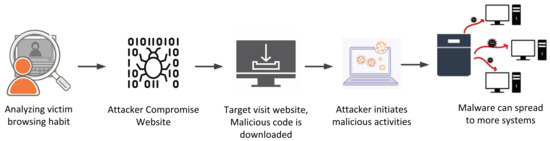
\includegraphics[width=0.75\linewidth]{waterhole.png}
     \caption{Figure 5.} Steps of a water hole attack.
     \label{fig:placeholder}
 \end{figure}
 
\paragraph{\textit{2.5. Reverse Social Engineering}}

Reverse engineering attacks are among the simplest yet most effective attack methods in SE attacks. Reverse engineering attacks are carried out in two steps. First, the malicious actor creates a problem for the target. The core idea behind the creation of the problem is to initiate an interaction with the target. Second, the malicious actor approaches the victim with the solution to that problem. For example, the foe identifies a potential target in an organization and intentionally creates a problem related to the information technology (IT) department. Later, the foe poses as a person from the IT department, or a benefactor, and offers assistance. Such acts are used to gain the trust of the intended target. With time, the malicious actor gains more trust and exploits the trust factor to gain sensitive information or manipulate the victim. Reverse engineering attacks are very common attacks at an organizational level.

\paragraph{\textit{2.6. Deepfake}}

Deepfake is a recent and highly convincing technique used to conduct SE attacks. Cybercriminals use deepfakes to forge images, audio, and video to achieve a particular goal. In cybersecurity, the deepfake is a growing threat. One of the most well-known algorithms for generating deepfake content is generative adversarial networks (GANs). GANs are a combination of two artificial neural networks (ANNs).These ANNs are called detectors and synthesizers. These ANNs are trained using large datasets of real images, audio, and video clips. Then, the synthesizer ANN generates deepfake content and the detector ANN attempts to distinguish the authenticity of the content. The cycle of generating deepfake content continues until the detector ANN is no longer able to identify the generated fake content as fake. Due to this rigorous process of generation and validation, the generated forged content by GAN is very difficult to identify as fake.  It can be seen that two different faces i.e., Face A and Face B are used to train a network. Later the network is used to generate Face A with expressions or audio from Face B. The newly generated image with the original Face-A interpretation by Face-B can be used to confuse or influence a victim. In  deepfake was employed for the SE attack conducted on a UK-based energy firm. In the attack, the deepfake voice was used to scam the CEO of the company [\href{https://www.mdpi.com/2076-3417/12/12/6042\#B15-applsci-12-06042}{\textbf{15}}]. Other than scamming, deepfake has also been used in several other criminal activities, i.e., blackmailing, damaging reputation, fake news, misinformation, mass panic, etc.


% \begin{figure}
     \justifying
     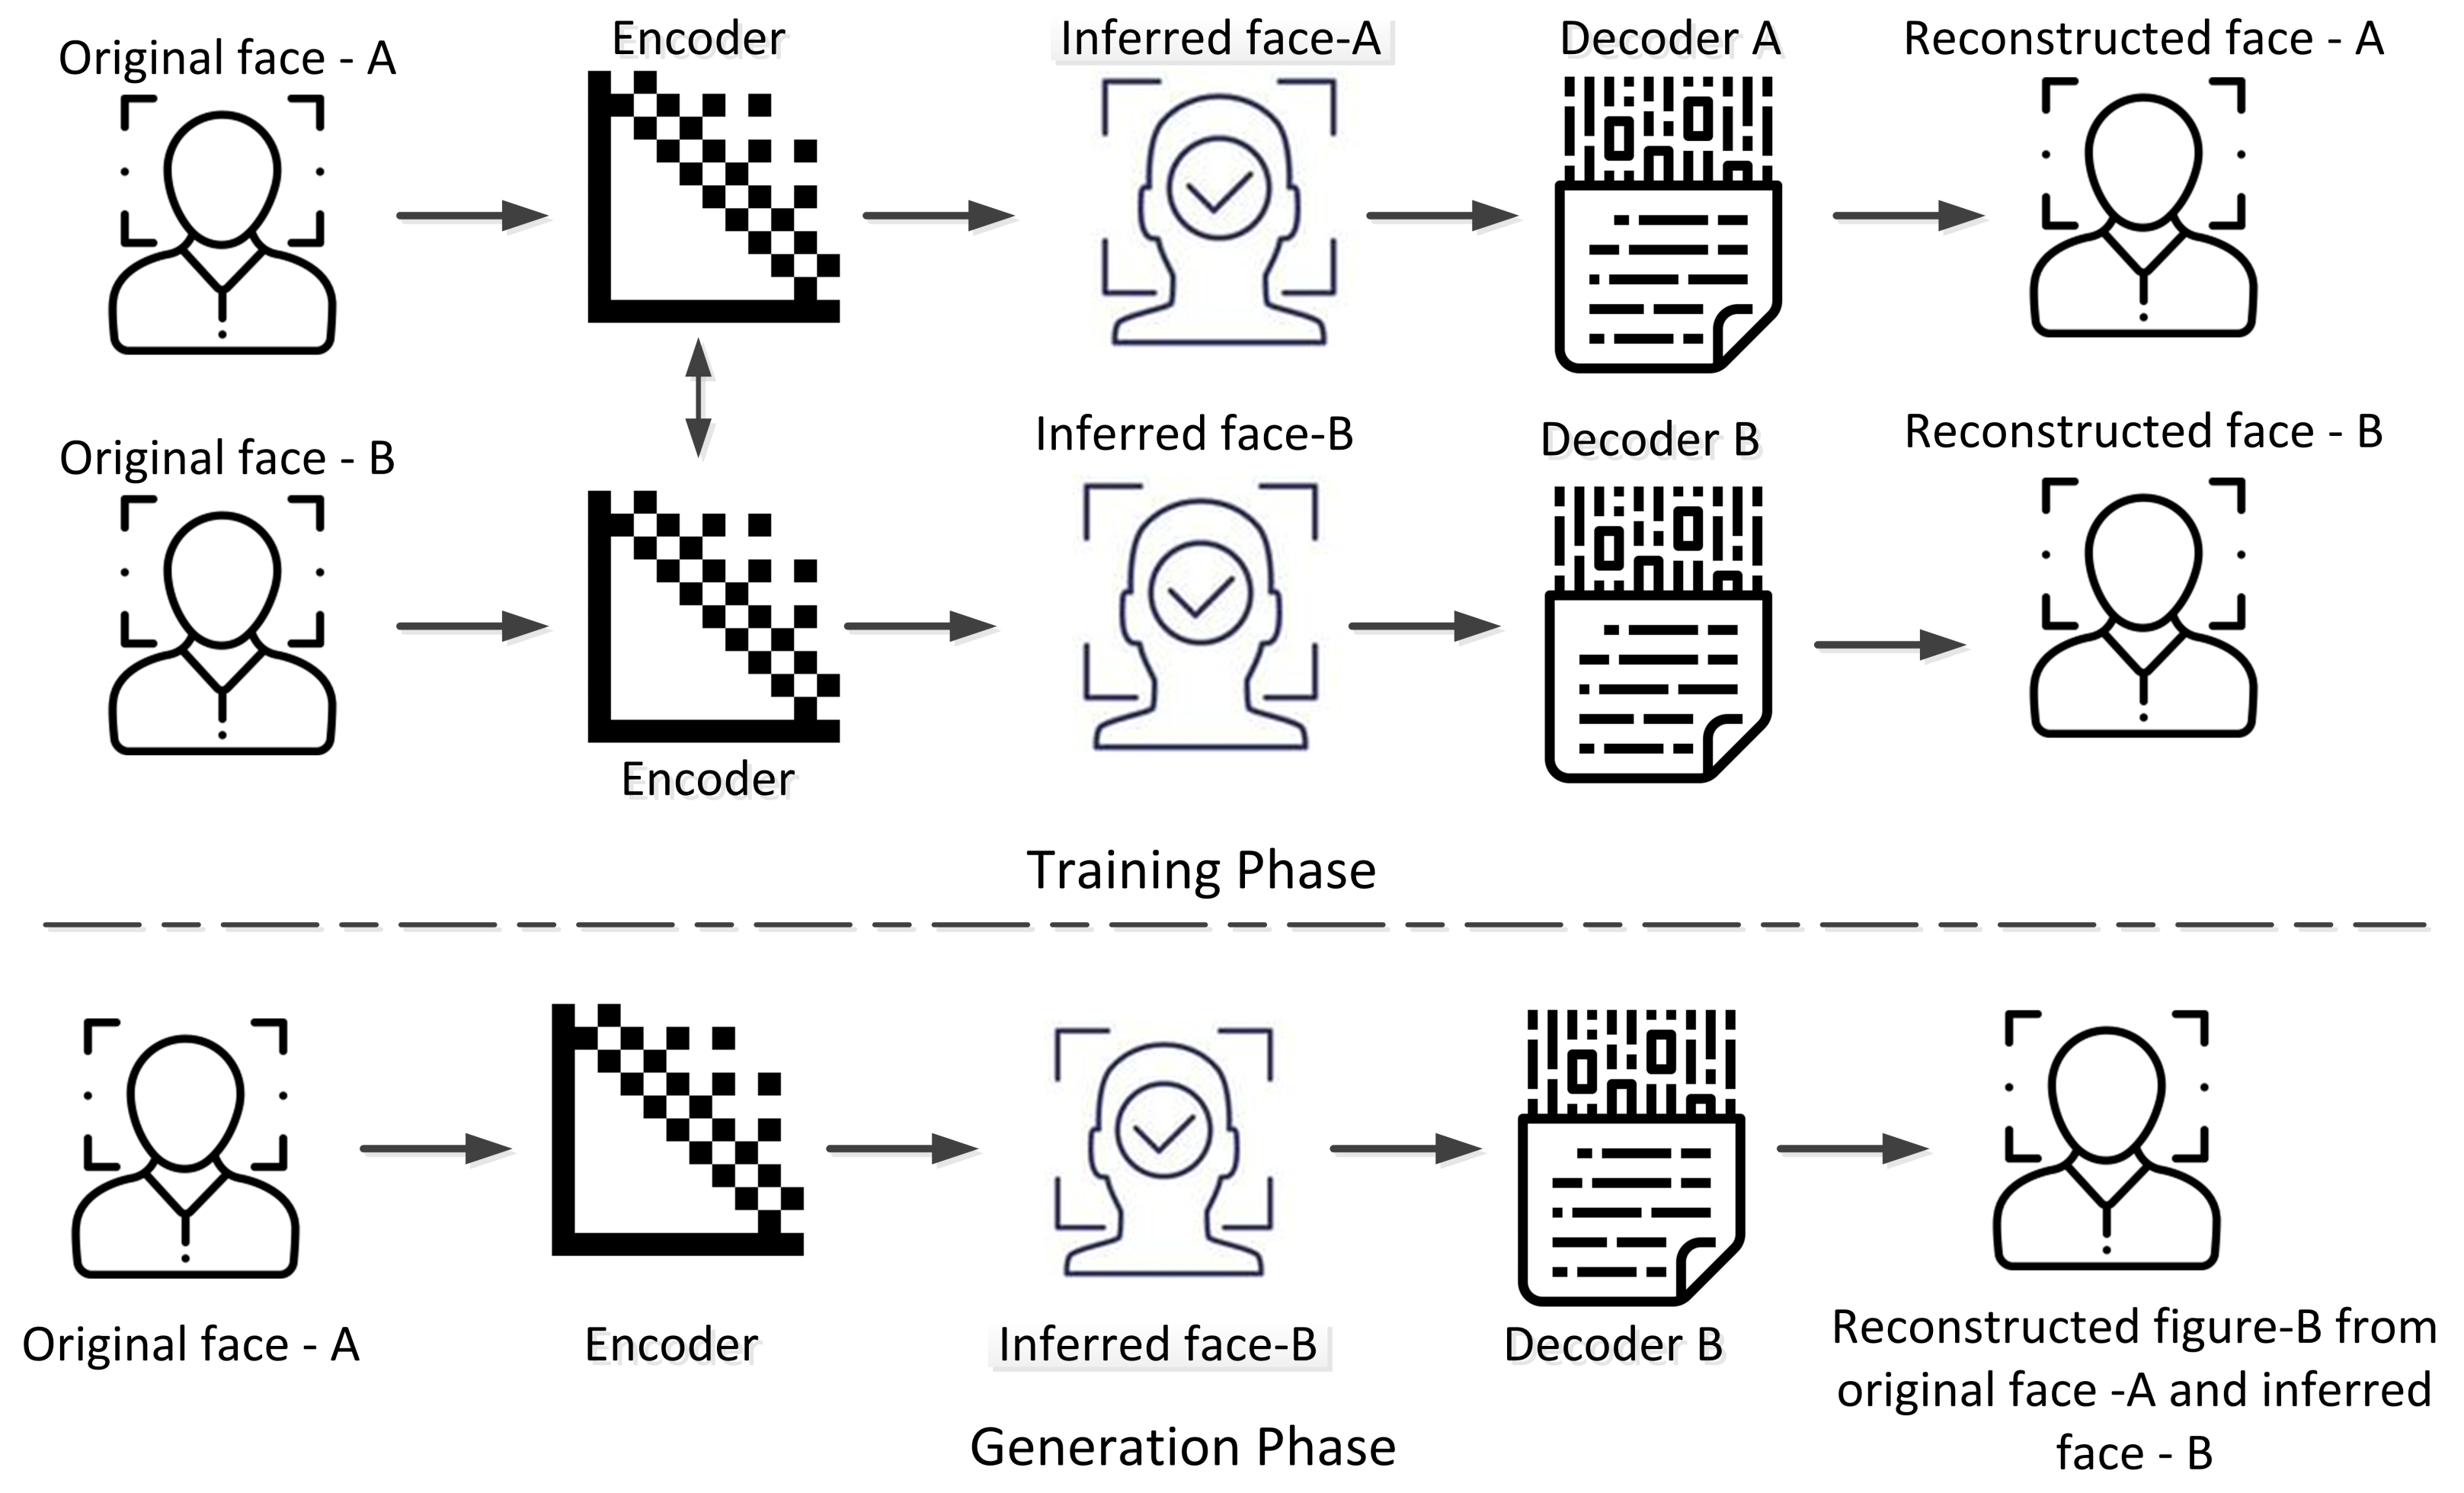
\includegraphics[width=0.75\linewidth]{deepfake.png}
 %    \caption{\textbf{Figure 6.} Simplified illustration of training and generating deepfake images or videos.
     \label{fig:placeholder}
% \end{figure}
 
\subsection{\textbf{3. Influence Methodologies}}

To initiate a SE attack, the attacker needs some form of influence on the target. This section discusses the different methods to influence and compromise a victim. The prominent human behavioral aspects that are used to initiate a SE attack are social influence, persuasion, attitude and behavior, trust, fraud, decision making, emotions, language, reasoning, etc. [\href{https://www.mdpi.com/2076-3417/12/12/6042\#B3-applsci-12-06042}{\textbf{3}}]. The mentioned behavioral aspects are also used in cyberattacks based on SE. Based on the victim attributes, the attackers exploit the most suitable human vulnerability. The attackers can also use multiple vulnerabilities at different stages of an attack.

\paragraph{\textit{3.1. Social Influence}}

Social influence includes both intentional and unintentional efforts to alter another person’s behavior or attitude. Usually, social influence works through peripheral processing. In such an approach, the victim may be unaware of the influence attempt by the attacker [\href{https://www.mdpi.com/2076-3417/12/12/6042\#B37-applsci-12-06042}{\textbf{37}}]. In general, social influences are categorized into three types utilitarian, value-expressive, and informational [\href{https://www.mdpi.com/2076-3417/12/12/6042\#B38-applsci-12-06042}{\textbf{38}}].Informational influence refers to the influence of an individual over a particular group. For example, while shopping, a member of a group suggests what to buy based on earlier ‘experience’ information. The utilitarian influence refers to the influence on an individual or a group based on a reward or something similar. Value expression influence is influence due to interests or beliefs. For instance, on social media, people join groups based on their hobbies and interests. To further elaborate on how these influence methods work, \href{https://www.mdpi.com/2076-3417/12/12/6042\#table_body_display_applsci-12-06042-t003}{\textbf{Table 3}} provides a more detailed look into social influence interlinked with SE attacks.

\textbf{Table 3.} Social influence methods related to cyberattacks based on social engineering.



 
\paragraph{\textit{3.2. Persuasion}}

Social engineering relies on persuasion methods to manipulate victims into performing actions or revealing confidential information. Persuasion is a well-known method that is used in several other domains, such as sales, marketing, insurance, and others. etc. [\href{https://www.mdpi.com/2076-3417/12/12/6042\#B44-applsci-12-06042}{\textbf{44}}]. As per Robert Cialdini [\href{https://www.mdpi.com/2076-3417/12/12/6042\#B45-applsci-12-06042}{\textbf{45}}], there are six main principles of persuasion—reciprocation, commitment and consistency, social proof, authority, liking, and scarcity. Reciprocation defines the behavior in which an individual replies to kindness with kindness. For example, if a coworker buys you lunch; you will feel obliged to buy him/her lunch the next time. A sense of commitment and consistency can be defined as a desire to be consistent with behavior. This behavior can include moral values, music, favorite food, etc. Social proof can be referred to as peer pressure. It refers to the intentional or unintentional acts of doing what everyone else is doing, (e.g., if a group is looking out of a window, anyone who sees them will also look out of the window). The principle of liking is simply the act of agreeing with people whom we like. Similarly, the principle of authority refers to the act or tendency of individuals to follow authority. The principle of scarcity refers to the approach of persuasion using time-based constraints. For example, limited-time sales are used to persuade potential buyers to buy products before time runs out and the product price is increased. These six principles play a key role in SE attacks that rely on persuasion. Further, \textbf{Table 4} highlights some of the persuasion methods used in conducting cyberattacks based on SE.

\textbf{Table 4.} Persuasion types used in social engineering attacks.
 
\paragraph{\textit{3.3. Attitude and Behavior}}

The theory of planned behavior (TPB) describes a psychological model to predict behavior. The TPB model can be seen in \textbf{Figure 7} [\href{https://www.mdpi.com/2076-3417/12/12/6042\#B52-applsci-12-06042}{\textbf{52}}]. The ‘attitude toward the behavior’ defines the motivation factors, i.e., the effort a person is willing to put in, to show a certain behavior. For example, an individual on social media might not be willing to share personal information but might participate in an online activity where privacy might be in significant danger. The ‘subjective norm’ defines an individual’s behavior influenced by his/her social circle. A person may align his/her behavior to be associated with a group. The ‘perceived behavior control’ indicates the level of control an individual has over a certain behavior. The three branches of TPB can be used to encourage a victim into revealing information based on the behavioral stimulus [\href{https://www.mdpi.com/2076-3417/12/12/6042\#B53-applsci-12-06042}{\textbf{53}}].
\begin{figure}
    \justifying
    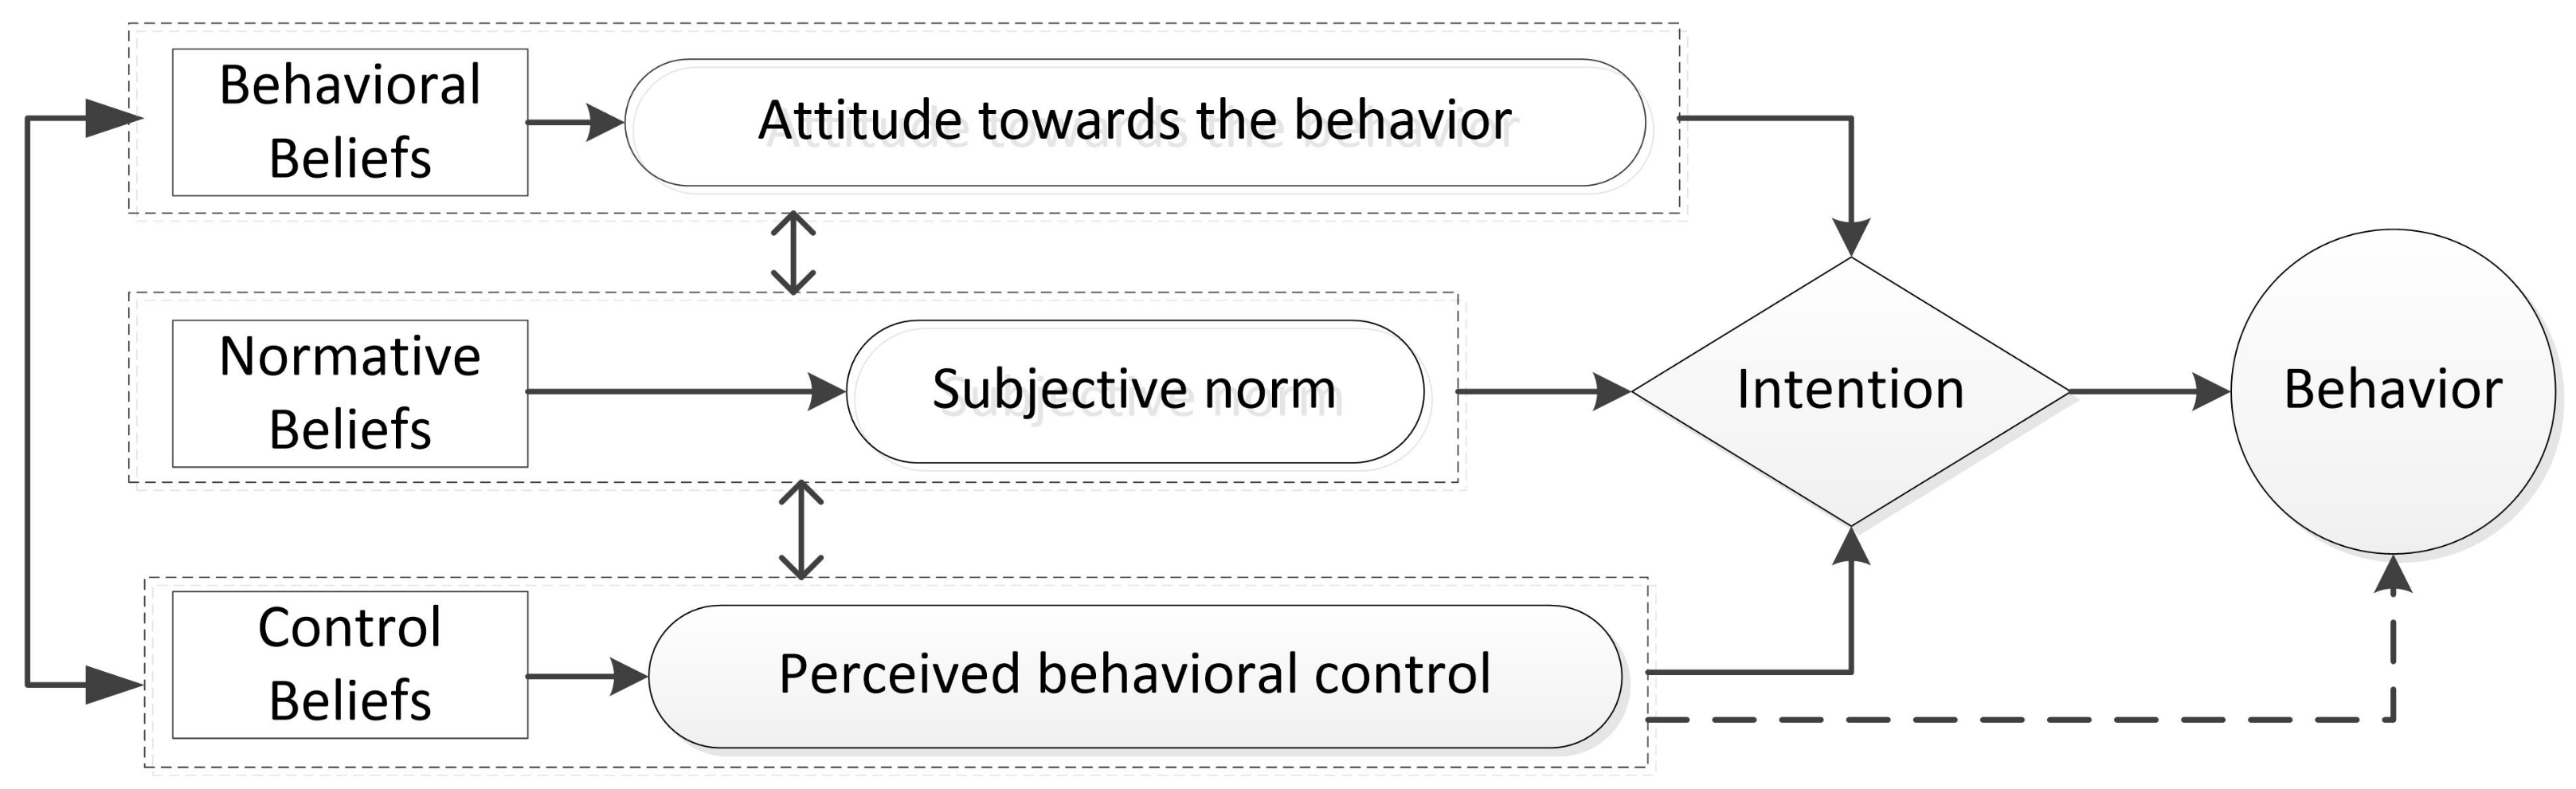
\includegraphics[width=0.75\linewidth]{theory.png}
    \caption{Figure 7.} Theory of planned behavior.
    \label{fig:placeholder}
\end{figure}

The methods to influence the attitudes and behaviors of victims can further be divided into subdomains, as shown below.

Subdomains of Trust and Deception

Trust is a cornerstone of human interaction-and deception is its calculated exploitation. In cybersecurity, especially in spearphishing and social engineering, attackers succeed not merely by exploiting technical vulnerabilities but by navigating, manipulating, and sometimes dismantling a target's trust framework. The subdomains of trust and deception refer to specific psychological, social, and contextual areas in which trust is built, maintained, and, at the same time, manipulated, and where deception can be most effective.

Understanding these subdomains is crucial for defenders because each represents a distinct attack vector. For attackers, these are leverage points-trust anchors that can be weaponized to bypass suspicion and encourage action. Some of the key psychological facets that social engineers exploit include, but are not limited to:

\subsection{1. Principles of Influence (Cialdini's Principles)}
\begin{itemize}
    \item Reciprocity
    \item Commitment and Consistency
    \item Social Proof
    \item Authority
    \item Liking
    \item Scarcity
\end{itemize}

\subsection{2. Emotional Manipulation}
\begin{itemize}
    \item Fear and Urgency
    \item Greed
    \item Curiosity
    \item Helpfulness / Sympathy
\end{itemize}

\subsection{3. Cognitive Biases}
\begin{itemize}
    \item \textit{Anchoring Bias}-Anchoring bias is the tendency for individuals to rely too heavily on the first piece of information they receive (the "anchor") when making subsequent judgments or decisions. Social engineers exploit this bias by presenting an initial piece of information, often misleading or irrelevant, to influence a target's perception and behavior.
    \item How It Works:
    \begin{itemize}
        \item \textit{1. The Initial Anchor:}
        \begin{itemize}
            \item A social engineer might start by presenting a high or low price for something, a fake statistic, or a fabricated piece of information.
        \end{itemize}
    \item \textit{2. Influence on Subsequent Decisions:}
    \begin{itemize}
        \item This initial "anchor" then influences how the target perceives and evaluates subsequent information or requests. For example, if a high initial price is presented, a subsequent lower price might seem like a good deal, even if it is still above the actual market value.
    \end{itemize}
    \item \textit{3. Skewed Perception:}
    \begin{itemize}
        \item By manipulating the initial anchor, social engineers can skew the target's perception of reality, making them more likely to accept their request to offers.
    \end{itemize}
    \end{itemize}
        \end{itemize}

\subsubsection{Examples of Anchoring Bias in Social Engineering}
\textbf{Negotiations:}
An attacker might start by suggesting an unrealistically high price for something, making a subsequent, more reasonable offer seem like a concession.

\textbf{Information Gathering:}
A social engineering might present a fake statistic about a company's performance to make a target more likely to divulge sensitive information that confirms that statistic.

\textbf{Phishing Attacks:}
An email that includes a large sum of money in the subject line might be an attempt to anchor the recipient's perception of the sender before asking for personal information.

\subsubsection{Guarding Against Anchoring Bias in Security Decisions}
When it comes to cybersecurity, users are often presented with information that can heavily influence their decisions. A common pitfall is anchoring bias-the tendency to rely too heavily on the first piece of information received, even when it may be incomplete or misleading. Training users to recognize and counter this bias is essential for building resilient security habits.

\textbf{Train users and staff to be aware of the bias:} Train users and staff to recognize that the first piece of information they receive might not be accurate or relevant. Research current red flags and and disseminate for user and staff situational awareness. 







Confirmation Bias
    \begin{itemize}
    \item Recency Bias
    \item Overconfidence Bias
    \item Halo Effect
    \item Commitment and Consistency
    \item Framing Effect

\end{itemize}

\subsection{4. Availability Heuristic}
    \begin{itemize}
        \item \textbf{Explanation:}People tend to overestimate the likelihood or importance of information that is easily recalled or readily available in their minds.
        \item \textbf{Social Engineering Exploitation:} Attackers leverage recent events, news stories, or familiar scenarios to make their attacks more believable and impactful. For example, referencing a recent data breach in a phishing email can increase the sense of urgency and make victims more likely to click on malicious links.
    \end{itemize}

\subsection{5. Loss Aversion}
\begin{itemize}
    \item \textbf{Explanation:}Individuals feel the pain of a loss more strongly than the pleasure of an equivalent gain.
    \item \textbf{Social Engineering Exploitation:} Attackers frame their messages in terms of potential losses if the target does not comply. For example, threatening account suspension or data deletion can be more effective than promising a reward (that can't ever be legitimately delivered).
\end{itemize}

\subsection{6. Hyperbolic Discounting}
\begin{itemize}
    \item \textbf{Explanation:} People prefer smaller, immediate rewards over larger, delayed rewards.
    \item \textbf{Social Engineering Exploitation:} Attackers offer immediate, seemingly attractive rewards to entice victims into making quick decisions without considering the long-term consequences. For example, offering a free gift or discount that requires personal information such as zip code or birth date can exploit this bias.

\end{itemize}

\subsection{7. Ostrich Effect}
\begin{itemize}
    \item \textbf{Explanation:} Individuals avoid information they perceive as negative or threatening, similar to the proverbial ostrich burying its head in the sand.
    \item \textbf{Social Engineering Exploitation:} Attackers create a sense of urgency by implying that if the target does not act quickly, something negative will happen. This pushes individuals to act before fully evaluating the situation.
\end{itemize}

\subsection{8. Optimism Bias}
\begin{itemize}
    \item \textbf{Explanation:} People tend to overestimate the likelihood of positive events occurring to them while underestimating the probability of negative events.
    \item \textbf{Social Engineering Exploitation:} Attackers might offer enticing but false opportunities like fake job offers or lottery winnings, playing on the target's optimism and desire for positive outcomes.
\end{itemize}

\subsection{9. Curiosity Effect}
\begin{itemize}
    \item \textbf{Explanation:} People are drawn to resolve uncertainty or curiosity, even if it might lead to negative consequences.
    \item \textbf{Social Engineering Exploitation:} Attackers use intriguing subject lines or offer "secret information" or exclusive deals to pique the target's curiosity and encourage them to click on malicious links or open infected attachments. 
\end{itemize}

\subsection{10. Ingratiation}

Correlating TPB Into Social Engineering Attacks

\subsection{\textbf{1. Attitude Toward the Behavior}}

\begin{itemize}
    \item \textbf{TPB Meaning:} A person’s evaluation of whether performing the behavior is good or bad.
    \item \textbf{Attacker’s Goal:} Make the \textit{malicious action} (clicking a link, opening an attachment, sharing credentials) seem beneficial, low-risk, or even necessary.
    \item \textbf{Exploitation Examples:}
    \begin{itemize}
        \item Framing the action as \textbf{helpful}: “We need your urgent input to finalize the quarterly report.”
        \item Creating a \textbf{positive reward association}: “You’ve won an award—click to claim it.”
        \item Downplaying risk: “This is just the updated company form, nothing sensitive.”
    \end{itemize}
\end{itemize}
\textbf{Defender’s Takeaway:} Security awareness must shift employees’ \textit{attitude} by making risky actions seem \textit{unambiguously negative} and reminding them of the potential harm.

\subsection{\textbf{2. Subjective Norms}}

\begin{itemize}
    \item \textbf{TPB Meaning:} The perceived social pressure to perform or not perform the behavior.
    \item \textbf{Attacker’s Goal:} Make the target believe that \textbf{important or respected people expect} them to comply—or that “everyone else is doing it.”
    \item \textbf{Exploitation Examples:}
    \begin{itemize}
        \item \textbf{Authority Impersonation:} “This is a direct request from the CEO.”
        \item \textbf{Social Proof:} “All team leads have already completed this step.”
        \item \textbf{Peer pressure framing:} “Finance already sent their details—why are you delaying?”
    \end{itemize}
\end{itemize}
\textbf{Defender’s Takeaway:} Organizations should normalize \textit{verification before action} as the “expected” social behavior, so the default pressure is to confirm legitimacy before complying.

\subsection{\textbf{3. Perceived Behavioral Control (PBC)}}

\begin{itemize}
    \item \textbf{TPB Meaning:} How capable the person feels in performing the behavior.
    \item \textbf{Attacker’s Goal:} Lower the target’s perception of difficulty so compliance feels effortless—or make refusal seem technically impossible.
    \item \textbf{Exploitation Examples:}
    \begin{itemize}
        \item Providing a \textbf{simple, frictionless path}: “Just click this one link and enter your password.”
        \item \textbf{Time pressure:} “This must be done within the hour or your account will be suspended,” removing time to think.
        \item Making it \textbf{feel routine}: “This is the same payroll confirmation process you’ve always used.”
    \end{itemize}
\end{itemize}
\textbf{Defender’s Takeaway:} Increase employees’ \textit{perceived control over resisting}—for example, by training them in easy verification techniques and creating low-friction reporting tools.

\subsection{\textbf{Putting It Together: The Attacker’s TPB Model}}

Attackers design social engineering campaigns to influence the \textbf{intention} to comply:

\begin{quote}
\textbf{Influence Attitude} → “This is good/necessary for me.”

 \textbf{Influence Subjective Norms} → “My boss/peers expect this.”

 \textbf{Manipulate PBC} → “This is easy for me to do; refusing isn’t worth it.”

\end{quote}

When \textbf{intention} is high, actual compliance (behavior) follows—whether that’s opening an attachment, transferring funds, or sharing credentials.

\subsection{\textbf{Defender Application}}

From a defensive standpoint, TPB can be flipped:

\begin{itemize}
    \item \textbf{Attitude:} Train staff to see \textit{non-compliance with suspicious requests} as positive.
    \item \textbf{Subjective Norms:} Make “verify first” a visible and valued norm in the culture.
    \item \textbf{PBC:} Give employees the tools and confidence to resist and report attacks.
\end{itemize}
If you’d like, I can \textbf{build a TPB-based “social engineering attack lifecycle” diagram} showing exactly how phishing emails or vishing calls are structured to target \textit{each TPB element} and push the victim toward compliance.

 That would make it easy to spot attacker patterns in real campaigns.



\subsection{1. Relational Trust}
\textbf{Description:} Relational trust arises from familiarity-personal relationships, known colleagues, repeated interactions, or established rapport. It is strongest when forged over time and reinforced by consistent, positive behavior.

\textbf{Deception Angle:} Attackers exploit relational trust by impersonating known individuals or entities. This could be via email spoofing, typosquatting, or even compromising legitimate accounts to send messages. Because the sender appears familiar, the target's cognitive guard lowers, making them more likely to comply first without even thinking to verify.

\textbf{Example:} An email from a "manager" requesting urgent document access. Even subtle cues-such as a familiar greeting style or referencing past projects-can anchor the deception.

\begin{svgraybox}
\textbf{Defensive Relevance:}

Defenders must educate users that even known senders can be spoofed or compromised. Verification protocols and multi-channel confirmation processes help to mitigate relational trust exploitation.
\end{svgraybox}

\subsection{2. Contextual Trust}
\textbf{Description:} This trust stems from messages or requests fitting neatly into the recipient's immediate environment, workflow, or current events. If a message "belongs" in the moment, it will be less likely to raise any suspicions.

\textbf{Deception Angle:} Spearphishers craft messages that align with ongoing projects, organizational events, personal circumstances, or familiarities. This can include referencing company meetings, seasonal activities, or urgent business timelines.

\textbf{Example:} An HR-themed phishing email sent during open enrollment season, or a "project update" request arriving in the middle of an actual project cycle.

\begin{svgraybox}
\textbf{Defensive Relevance}
Security teams and defenders can deploy behavioral monitoring and timing awareness to detect anomalous patterns. For example, HR communications coming from non-HR domains.
\end{svgraybox}

\subsection{3. Authority-Based Trust}
\textbf{Description:} This form of trust is built on perceived power, expertise, or hierarchical status. Humans are more likely to comply with requests from those they believe have any type of authority or power over them.

\textbf{Deception Angle:} Attackers often impersonate law enforcement (\textbf{illegal} to do so, by the way), executives, senior staff, or recognized experts, issuing directives that appear urgent in nature and unquestionable. The "CEO Fraud" scam is a textbook example, where attackers instruct employees to transfer funds or disclose sensitive information.

\textbf{Example:} An email from the company CFO instructing a wire transfer, invoking urgent deadlines and the strictest confidentiality.

\begin{svgraybox}
    \textbf{Defensive Relevance:}

    Defenders must instill the importance into security teams to train employees to validate authority requests through secondary channels, especially those involving financial or data transfers. Implement dual-authorization or a double-verification for sensitive transactions.
\end{svgraybox}

\subsection{4. Procedural Trust}
\textbf{Description:} Procedural trust emerges when an interaction follows an expected and familiar process. If the request aligns with established protocols, it feels legitimate.

\textbf{Deception Angle:} Attackers mimic legitimate processes, such as forms, document templates, login flows, and more to convince targets that the request is standard procedure.

\textbf{Example:} A phishing page replicating the exact look and flow of the company's VPN login portal, or a fake "password reset" request using identical corporate branding schemes.

\begin{svgraybox}
    \textbf{Defensive Relevance:}
    Multi-factor authentication and verification alerts can interrupt procedural mimicry. Routine internal audits should look for cloned or spoofed instances.
\end{svgraybox}

\subsection{5. Social Proof Trust}
\textbf{Description:} Social proof occurs when people look to the actions of others to guide their own decisions, especially under uncertainty.

\textbf{Deception Angle:} Attackers create the illusion that others have already complied or endorsed the request. This can involve fabricating testimonials, references to specific group actions, or even displaying fake counters showing just how "many others" have acted.

\textbf{Example:} \textit{"Several colleagues have already completed this security update, we're just waiting for you to complete yours. Please click here to finalize your security update."}

\begin{svgraybox}
Defensive Relevance:
Users should be trained to recognize fabricated consensus claims and to verify the authenticity of group endorsements.
\end{svgraybox}

\subsection{6. Cognitive Ease and Habit Trust}
\textbf{Description:} Cognitive ease comes from familiarity, repetition, and simplicity. When something feels familiar and is easy to process, the brain perceives it as more trustworthy.

\textbf{Deception Angle:} Attackers exploit routine behaviors-such as clicking familiar-looking links or opening standard document formats. By replicating the "look and feel" of past legitimate communications, they reduce the mental friction that triggers skepticism.

\textbf{Example:} A monthly "invoice" notification from a supplier-except the sender's domain is subtly altered (e.g., legitimate = www.poolsupplies.com / illegitimate = www.poolsuplies.com/).

\begin{svgraybox}
\textbf{Deception Relevance:}
Break habitual click patterns with periodic simulated phishing and dynamic email banners that highlight potential risks.
\end{svgraybox}

\subsection{7. Reciprocity-Based Trust}
\justifying
\noindent\textbf{Definition: }Humans are wired to return favors and match perceived generosity or effort.
{\justifying
\par\noindent\textbf{Deception Angle}: Attackers offer something-information, a free tool, a perceived benefit-and expect the target to "give back" by clicking a link or providing access.} \\
{\justifying
\textbf{Example:} \textit{"As a valued employee, you have been given access to our new HR benefits portal."}}

%\begin{svgraybox}
\tipbox{Defensive Relevance:}
    Encourage healthy skepticism around unsolicited offers, even if they appear to come from legitimate internal sources.

\subsection{7. Reciprocity-Based Trust}
{\justifying
\noindent\textbf{{Definition:} }Temporal trust emerges when timing aligns perfectly with expectations or urgency creates a pressure to act quickly.}
{\justifying
\par\noindent\textbf{\textbf{Deception Angle:} }Deadlines, expiring offers, and emergency situations short-circuit rational decision-making. The perceived cost of delay outweighs the urge to verify authenticity.}
{\justifying
\textbf{\textbf{Example:}} \textit{"Your account will be locked in 24 hours unless you reset your password immediately."}}




\subsection{8. Temporal Trust}
\textbf{



\begin{svgraybox}
    \textbf{Defensive Relevance:}
    Educate users about urgency traps and encourage deliberate pause-and-verify practices-especially for requests with time pressure or constraints.
\end{svgraybox}


\subsection{Domains of Trust and Deception is Social Engineering}
\begin{quote}
    \textit{Trust is the grease of human interaction-and deception is the calculated contamination of that grease. In cybersecurity, particularly in spearphishing and social engineering, attackers succeed not only by exploiting technical vulnerabilities, but by infiltrating, manipulating, and dismantling a target's trust framework. Trust is not a monolith-it is composed of multiple psychological, social, and contextual elements, each of which can be targeted as a distinct attack surface.}
\end{quote}
Understanding these \textbf{subdomains of trust} is critical for defenders because it represents a unique \textbf{vector of manipulation.} For attackers, these are attractive leverage points-the "trust anchors" that can be weaponized to bypass suspicion and elicit an immediate action. Each subdomain below combines elements of \textbf{psychology, social dynamics, and behavioral economics,} along with the \textbf{cognitive biases} and \textbf{principles of influence} that make them effective.

\subsection{1. Relational Trust}
\textbf{Definition:} Built on familiarity and personal connection-colleagues, friends, long-term business relationships-strengthened by repeated positive interactions.
\textbf{Exploitation:} Social engineers impersonate known individuals, clone profiles, or compromise legitimate accounts. Subtle cues like tone, nicknames, or references to shared experiences lower the target's guard.
\textbf{Example:} An email from a manager requesting sensitive files, signed with their usual salutation and referencing last week's meeting.
\textit{"Hey, it's Nick from accounting-can you please send me the vendor payment files from last week? I'm swamped and just need to forward them to finance before the meeting."}
\textbf{Bias / Principle Link:} \textit{Liking, Similarity, Halo Effect.}
\textbf{Defensive Relevance:} Train employees that "familiar" is not "safe." Use multi-channel verification and account-compromise monitoring.

\subsection{2. Contextual Trust}
\textbf{Definition:} Arises when a request fits neatly into the target's current work, environment, or life context.
\textbf{Exploitation:} Attackers time messages to align with seasonal events (tax season, open enrollment) or active projects, making them seem naturally embedded in ongoing activities.
\textbf{Example:} A fake HR survey during benefits enrollment week.
\textit{"Hi, we are finalizing the open enrollment forms today as it is the deadline. Can you please log into the HR portal and confirm your benefits selections before 5 pm?"}
\textbf{Bias / Principle Link:} \textit{Framing Effect, Availability Heuristic.}
\textbf{Defensive Relevance:} Flag unexpected senders or domains in time-sensitive processes. Build awareness of "contextual mirroring" as a red flag.

\subsection{3. Authority-Based Trust}
\textbf{Definition:} Trust granted due to hierarchical status, power, or perceived authority or expertise.
\textbf{Exploitation:} "CEO fraud" and law enforcement impersonation prey on obedience to authority and fear of repercussions.
\textbf{Example:} A spoofed email from the CFO ordering a confidential wire transfer.
\textit{"This is Nina from the CFOs office. The CEO needs these wire transfers processed immediately for a confidential acquisition-send the confirmation once its done."}
\textbf{Bias / Principle Link:} \textit{Authority, Obedience Effect.}
\textbf{Defensive Relevance:} Implement dual-authorization for high-risk actions; normalize questioning authority in digital requests.

\subsection{4. Procedural Trust}
\textbf{Definition:} Rooted in familiarity with established processes and workflows.
\textbf{Exploitation:} Attacker replicate standard forms, login flows, and reset processes to create the illusion of legitimacy.
\textbf{Example:} A phishing page mimicking the exact look and URL structure of the corporate VPN portal.
\textit{"Hi, this is your IT department. We have noticed a login issue with your corporate VPN account. At your earliest convenience, please reset your password using the standard portal link provided below to avoid being locked out or having your account suspended."}
\textbf{Bias / Principle Link:} \textit{Cognitive Ease, Commitment and Consistency.}
\textbf{Defensive Relevance:} Use unique visual indicators for genuine information systems; audit for lookalike or typosquatted domains.

\subsection{5. Social Proof Trust}
\textbf{Definition:} Trust generated by the perception that "everyone else" is doing something.
\textbf{Exploitation:} Messages claim that colleagues have already complied or that the request is standard practice.
\textbf{Example:} "All team leads have already completed this mandatory security step-we are just waiting on yours."
\textbf{Bias / Principle Link: }\textit{Social Proof, Normative Influence.}
\textbf{Defensive Relevance:} Teach employees to verify claims of group participation through official channels.

\subsection{6. Cognitive Ease and Habit Trust}
\textbf{Definition:} Comfort and lowered skepticism for repetition and familiarity.
\textbf{Exploitation:} Malicious requests mimic routine tasks-invoice approvals, meeting invites-to slip past mental defenses.
\textbf{Example:} A monthly "invoice" with a slightly altered sender domain.
\textbf{Bias / Principle Link:} \textit{Recency Bias, Anchoring Bias.}
\textbf{Defensive Relevance:} Introduce controlled variability into routine processes; run simulations to break autopilot behaviors.

\subsection{7. Reciprocity-Based Trust}
\textbf{Definition:} The human tendency to return favors and match perceived generosity.
\textbf{Exploitation:} Attackers offer perks, early access, or helpful information in exchange for action.
\textbf{Example:} "As a valued employee, you have early access to our new HR portal."
\textbf{Bias / Principle Link:} \textit{Reciprocity Principle.}
\textbf{Defensive Relevance:} Encourage skepticism toward unsolicited "benefits," even when internally branded.

\subsection{8. Temporal Trust}
\textbf{Definition:} Trust (and compliance) heightened when timing matches expectations or urgency limits decision-making.
\textbf{Exploitation:} Urgency framing ("Your account will be locked in 24 hours") forces fast action without verification.
\textbf{Example:} A fake "final warning" about account suspension.
\textbf{Bias / Principle Link:} \textit{Scarcity, Loss Aversion, Hyperbolic Discounting.}
\textbf{Defensive Relevance:} Teach deliberate pause techniques; enforce mandatory cooling-off periods for certain actions to gain a "clearer mind."

\subsection{9. Emotional Leverage}
\textbf{Definition:} Trust shaped or overridden by emotional state-positive or negative.
\textbf{Exploitation:} Fear, greed, curiosity, or flattery can override rational analysis.
\begin{itemize}
    \item \textbf{Fear / Urgency:} Threats of loss or negative outcomes (\textit{Loss Aversion, Ostrich Effect})
    \item \textbf{Greed:} Promises of financial gain or rewards. (\textit{Optimism Bias})
    \item \textbf{Curiosity:} Teasing "secret" or "exclusive" information. (\textit{Curiosity Effect})
    \item \textbf{Ingratiation / Flattery:} Boosting the target's self-image (\textit{"You are the only one I trust to do this right"}). (\textit{Liking, Social Exchange Theory})
\textbf{Example: }"You have been selected for an exclusive leadership program-click now to confirm participation."
\textbf{Defensive Relevance:} Include emotional manipulation recognition in training; rehearse slow-response decision-,making under emotional load.
\end{itemize}

\subsection{10. Cognitive Bias Exploitation}
Beyond the subdomains above, attackers systematically weaponize \textbf{predictable thinking shortcuts:}
\begin{itemize}
    \item \textbf{Anchoring Bias:} Setting a mental reference point to influence decisions.
    \item \textbf{Confirmation Bias:} Supplying information that aligns with the target's existing beliefs.
    \item \textbf{Halo Effect:} Borrowing trust from one attribute (e.g., professional appearance) to mask malicious intent.
    \item \textbf{Framing Effect:} Presenting the same choice in gain versus loss terms to steer compliance initiatives.
\end{itemize}
\textbf{Defensive Relevance:} Bias-awareness training can help users pause before acting when a message "feels right" without evidence.

\subsection{11. Theory of Planned Behavior (TPB) in Social Engineering}
Attackers map their strategies to TPBs three levers:
\begin{itemize}
    \item \textbf{Attitude Toward the Behavior:} Make malicious actions seem beneficial or harmless.
    \item \textbf{Subjective Norms:} Suggest that respected figures or peers expect compliance.
    \item \textbf{Perceived Behavioral Control:} Remove perceived obstacles to acting; make refusal seem costly or impossible.

\end{itemize}

\subsection{12. Ingratiation (Ego-Boosting / Flattery)}
\textbf{Mechanism:} You create rapport and lower skepticism by appealing to the target's self-esteem, ego, or sense of uniqueness. By flattering their skills, reliability, or importance, you make them feel valued and special-thereby increasing the likelihood they will comply with your request.
\textbf{Typical Phrases:}
\begin{itemize}
    \item \textit{"You're the only one I can trust with this."}
    \item \textit{"You are my go-to person for this kind of thing."}
    \item \textit{"Nobody else has the expertise that you do."}
\end{itemize}
\textbf{Why It Works:}
\begin{itemize}
    \item \textbf{Reciprocity Trigger:} People often feel a subconscious need to "return the favor" after being given praise.
    \item \textbf{Self-Concept Alignment:} The request aligns with how they want to see themselves-competent, trusted, essential.
    \item \textbf{Reduced Critical Thinking and Rationale:} Positive emotional states, especially pride, can reduce vigilance and increase compliance.
\end{itemize}
\textbf{Psychological Foundations:}
\begin{itemize}
    \item \textbf{Cialdini's Principle of Liking:} We are more easily persuaded by people who express admiration for us.
    \item \textbf{Ego Depletion Effect:} Ego-boosting can shift focus away from skepticism toward maintaining the positive interaction.
    \item \textbf{Ingratiation Theory:} Strategic praise increases perceived similarity and rapport, leading to greater compliance.
\end{itemize}







By aligning with these levers, attackers raise the intention to comply, which directly increases the likelihood of the target performing the malicious action.

The subdomains of trust and deception are not isolated-attackers often blend multiple laevers in a single communication. An email could simultaneously exploit \textit{authority, context, urgency,} and \textit{social proof.} Defenders must train to recognize these patterns in combination, not in isolation, and develop layered verification and cultural norms that erode the attacker's psychological foothold.


\begin{itemize}
    \item Trust / Relation
    \begin{itemize}
        \item Building trust is one of the most crucial parts of an SE attack. An attacker can use multiple means to develop a trusted
    \end{itemize}
\end{itemize}








\paragraph{\textit{3.5. Language and Reasoning}}

Language is not only the most common method of communication, but it is also a means of processing, generating, and expressing thoughts. The process of social interaction using language is very similar to a programming language process. Humans hear the words as input, process those words, and generate a response as output. Seeking appropriate words to explain the context of the subject or feeling is important. This implies that crafting and elaborating information for SE attacks relies heavily on the language being used for interacting with the victim, i.e., the language cognition is exploited. \textbf{Table 7} provides an overview of language and reasoning sub-domains associated with SE attacks.\textbf{Table 7.} Sub-domains of language/reasoning linked with social engineering attacks.Effective cyberattacks based on SE rely on human vulnerabilities. The attackers exploit human behavior, knowledge, emotions, cognition, personal traits, human nature, etc. \textbf{Table 8} highlights the human vulnerabilities associated with SE attacks. A single SE attack can be conducted using multiple influence methods. A single influence method can exploit several human vulnerabilities. This multidimensional interconnection between SE attacks, influence methods, and human vulnerabilities makes SE-based cyberattacks challenging for security professionals.\textbf{Table 8.} Association between social engineering-based cyberattacks, method of influence, and human vulnerability.The mapping in \href{https://www.mdpi.com/2076-3417/12/12/6042\#table_body_display_applsci-12-06042-t008}{\textbf{Table 8}} provides a simple yet elaborate perspective on the working of SE attacks. Such mapping can assist greatly in identifying the vulnerabilities and building an effective security infrastructure to mitigate them. The highlighted interconnection between human vulnerabilities and SE attacks may not be sufficient to represent every age group or human behavior; however, it can provide a broader perspective to individuals and organizations on understanding and countering these SE-based cyberattacks.

\paragraph{\textit{3.6. Countering Social Engineering-Based Cyberattacks}}

Human awareness can be identified as a key factor in countering SE attacks. SE methods focus on hacking humans by targeting human cognitive biases rather than machines. The methods to counter SE-based cyberattacks can be seen in \href{https://www.mdpi.com/2076-3417/12/12/6042\#table_body_display_applsci-12-06042-t009}{\textbf{Table 9}}. The ML-based approaches to counter and detect SE-based cyberattacks are discussed separately in \href{https://www.mdpi.com/2076-3417/12/12/6042\#sec5-applsci-12-06042}{\textbf{Section 5}}. Based on recently published work, most researchers find the following methods to be highly effective to counter SE attacks. Based on \href{https://www.mdpi.com/2076-3417/12/12/6042\#table_body_display_applsci-12-06042-t009}{\textbf{Table 9}}, it can be concluded that training and educating individuals on cybersecurity and SE attacks can play a significant role. In \href{https://www.mdpi.com/2076-3417/12/12/6042\#table_body_display_applsci-12-06042-t009}{\textbf{Table 9}}, the checkmark highlight the countermeasures suggested by the referred study.\textbf{Table 9.} Suggested method to counter social engineering attacks.Several researchers have highlighted the role of well-defined policies to counter cyberattacks. Policies that can be implemented to avoid and manage an event of a data breach or SE-based cyberattacks. Organizational policies are further categorized into two main groups cybersecurity and communication policies. Cybersecurity policies are defined specifically for cyberattacks. Such policies may include instructions on avoiding illegal software, use of personal devices on the company network, steps to follow in case of cyberattacks, documentation of a cyberattack, human resources (HR) procedures for third party vendor privileges and access, critical area access management, password management, organizational security infrastructure, etc.A well-defined cybersecurity policy can limit many data breaches or cyberattacks. Moreover, organizational policies for official (or in some cases, unofficial) communication should be implemented. The reason to implement a separate set of policies for communication is based on the high number of SE attacks that exploit communication norms to conduct cyberattacks (i.e., \href{https://www.mdpi.com/2076-3417/12/12/6042\#table_body_display_applsci-12-06042-t001}{\textbf{Table 1}}). An organization should define clear policies for official communication within and outside the organization. Such policies may include a process of approval and validation for connecting a personal device to the organizational network, what level of information can be shared on emails, SMS, or calls, procedures to validate the authenticity of suspicious email, SMS, or calls, communication methods in case of working from home, etc. Organizational communication policies can play an integral role in avoiding any cyberattack based on SE. The importance and need of appropriate anti-viruses, firewall, spam filters, and updated software patches cannot be underestimated and must be installed on both organizational and personal systems. Some of the research and survey chapters on SE attack mitigation have encouraged organizations to provide company equipment to employees, as equipment managed by the organization’s IT department can easily be updated with security software and can be checked frequently for malicious software. Due to recent advancements in ML, the ML-based approaches are discussed separately in the following section.

\paragraph{\textit{3.7. Machine Learning-Based Countermeasures}}

Machine learning (ML) is another domain that can play an important role in countering SE-based cyberattacks. For phishing-based attacks, ML models can be trained to identify patterns and language in emails, SMS, malicious links, and even calls using natural language processing (NLP) [\href{https://www.mdpi.com/2076-3417/12/12/6042\#B58-applsci-12-06042}{\textbf{58}},\href{https://www.mdpi.com/2076-3417/12/12/6042\#B71-applsci-12-06042}{\textbf{71}}]. However, the continuous evolution of phishing characteristics can be a concern for ML-based methods. In this section, some of the most significant ML methods to counter SE-based cyberattacks are presented. The section also highlights the existing concerns with the discussed ML methods.

\paragraph{3.7.1. Deep Learning}

Deep learning (DL)-based approaches can also play a vital role in countering SE-based cyberattacks since DL has been an effective approach used to counter a wide range of malware, phishing attacks, traffic analysis, spam detection, intrusion detection, etc.. For instance, deep neural networks (DNNs) in DL are inspired by the human brain. As more data are fed to a DNN, it gradually becomes better at detecting malicious dialog. Due to this reason, Google is also using neural networks to detect spam emails. When it comes to phishing, DNN-based solutions can be highly effective. 

In, the authors proposed a hybrid model based on DNN and long short-term memory (LSTM) to identify phishing web links. The authors used NLP to select features and character embedding-based features for the DNN-LSTM model to identify phishing website links. The model was trained on two datasets—Ebbu2017 and a secondary dataset that was based on several internet resources. Even with the high detection rate by the proposed model, the authors stated the concerns on the datasets used. The datasets used may lack the precise representation of real work attacks. The chapters [\href{https://www.mdpi.com/2076-3417/12/12/6042\#B88-applsci-12-06042}{\textbf{88}},\href{https://www.mdpi.com/2076-3417/12/12/6042\#B89-applsci-12-06042}{\textbf{89}}] also presented DL-based approaches to counter SE-based attacks initiated through Twitter, DNS, URL, and email. The authors presented elaborate insight into the origination of ransomware based on different case studies. However, the absence of datasets representing sophisticated SE-based attacks may hold the key to enhanced DL to counter SE-based cyberattacks. This concern is highlighted by K. Simar, et al. in [\href{https://www.mdpi.com/2076-3417/12/12/6042\#B90-applsci-12-06042}{\textbf{90}}]; in their study, they presented a DL-based approach to structure the unstructured data generated by different internet sources. However, handling misinformation can be a concern in the proposed approach. When validating the authenticity of the source, publishing an event or article may still be questionable. Nonetheless, if the source validation process can be enriched, the proposed approach can play an integral role in improving the DL-based approach against SE attacks.

\paragraph{3.7.2. Reinforcement Learning}

Reinforcement learning (RL), another aspect of ML, is also a method used to counter SE-based cyberattacks. In [\href{https://www.mdpi.com/2076-3417/12/12/6042\#B91-applsci-12-06042}{\textbf{91}}], the authors proposed a cyber-resilient mechanism (CRM) to counter online threats, including uncertain real-time scenarios. The model used the feedback architecture of RL to define policies, as the system observes the online actions. However, the model requires online observations to learn and adapt unknown attack methods used in SE-based cyberattacks. In [\href{https://www.mdpi.com/2076-3417/12/12/6042\#B92-applsci-12-06042}{\textbf{92}}], the authors used the RL-based greedy approach. The authors used predefined attack and defense approaches (i.e., Petri net) to train the RL model. Based on the experimentation results, the authors concluded that the model gradually improved its performance to identify a cyberattack. The goal of the chapter was to highlight the potential of RL to counter cyberattacks. The main concern for the RL-based approach is the observation of an unlimited range of human behaviors. As time goes by, the data related to human behavior will grow exponentially, making it difficult to track and store information [\href{https://www.mdpi.com/2076-3417/12/12/6042\#B93-applsci-12-06042}{\textbf{93}}].

\paragraph{3.7.3. Natural Language Processing}

One of the most convenient tools in ML to counter phishing-based cyberattacks is NLP [\href{https://www.mdpi.com/2076-3417/12/12/6042\#B94-applsci-12-06042}{\textbf{94}}]. NLP with ML has played an important role in countering phishing attacks [\href{https://www.mdpi.com/2076-3417/12/12/6042\#B95-applsci-12-06042}{\textbf{95}}]. Several NLP processes, e.g., information extraction, text categorization, and machine translation, are inspired by DL [\href{https://www.mdpi.com/2076-3417/12/12/6042\#B96-applsci-12-06042}{\textbf{96}}]. The NLP relies on five main features to identify phishing emails or online links. Those features are email body characteristics, email subject, uniform resource locator (URL) characteristics, hidden script (i.e., JavaScript, pop-up on click activity, etc.) characteristics, and sender characteristics. A chapter by Tim Repke et al. [\href{https://www.mdpi.com/2076-3417/12/12/6042\#B97-applsci-12-06042}{\textbf{97}}] used the word-embedded technique with DL to analyze email text for human mode identification. This technique is not used to identify phishing, but it can be useful for identifying abnormalities in the usual email text, which can help in identifying email phishing, i.e., impersonation, BEC, clone phishing, etc. The only concern for the ML-based NLP model is the dependency on the surface text of an email. If the structure of dialog or a sentence is altered, it becomes difficult for the model to identify as phishing [\href{https://www.mdpi.com/2076-3417/12/12/6042\#B96-applsci-12-06042}{\textbf{96}}]. However, the key challenge for ML to counter SE-based cyberattacks is the absence of an attack pattern or a methodology that can identify the multidimensional approach to SE-based cyberattacks [\href{https://www.mdpi.com/2076-3417/12/12/6042\#B86-applsci-12-06042}{\textbf{86}}]. As discussed in \href{https://www.mdpi.com/2076-3417/12/12/6042\#sec3-applsci-12-06042}{\textbf{Section 3}}, SE-based attacks exploit human vulnerabilities, taking them beyond traditional security approaches in computer science. Therefore, the psychological decision-making and cognitive biases involved in SE-based cyberattacks are ongoing concerns for ML-based approaches . To achieve a higher detection rate, the researcher should explore the linguistic features of SE and integrate cognitive and psychological factors into ML-based approaches.

\subsection{\textbf{4. Discussion}}

The manipulation of human behavior and emotions in cyberattacks presents an unknown and challenging variable for security experts. The prime reason behind this variable can generally be characterized as culture. Culture can play an important role in influencing human behavior, beliefs, morals, decisions, and attitudes [\href{https://www.mdpi.com/2076-3417/12/12/6042\#B99-applsci-12-06042}{\textbf{99}},\href{https://www.mdpi.com/2076-3417/12/12/6042\#B100-applsci-12-06042}{\textbf{100}}]. Even with technological advancements in security, humans can be exploited for their vulnerabilities. Based on \href{https://www.mdpi.com/2076-3417/12/12/6042\#table_body_display_applsci-12-06042-t009}{\textbf{Table 9}}, it can be concluded that the most recent publications agree that raising the awareness of cybersecurity through training and education is essential. Such awareness can help in decreasing cyberattacks based on SE. On the other hand, some studies [\href{https://www.mdpi.com/2076-3417/12/12/6042\#B101-applsci-12-06042}{\textbf{101}},\href{https://www.mdpi.com/2076-3417/12/12/6042\#B102-applsci-12-06042}{\textbf{102}},\href{https://www.mdpi.com/2076-3417/12/12/6042\#B103-applsci-12-06042}{\textbf{103}}] highlight that despite appropriate training and policies, human vulnerabilities can still be exploited via SE attacks. For example, not every individual working in an organization has basic knowledge of computer security. Training an employee with no prior computer knowledge can be costly, time-consuming, and may not be very effective [\href{https://www.mdpi.com/2076-3417/12/12/6042\#B104-applsci-12-06042}{\textbf{104}}]. Such employees are highly vulnerable to several phishing-based SE attacks. Another study [\href{https://www.mdpi.com/2076-3417/12/12/6042\#B105-applsci-12-06042}{\textbf{105}}] concluded that an individual’s self-efficiency also plays an important role in avoiding SE attacks. The connection between an individual’s self-efficiency and vulnerability to SE attacks is further explored in some research publications.chapters [\href{https://www.mdpi.com/2076-3417/12/12/6042\#B1-applsci-12-06042}{\textbf{1}},\href{https://www.mdpi.com/2076-3417/12/12/6042\#B4-applsci-12-06042}{\textbf{4}},\href{https://www.mdpi.com/2076-3417/12/12/6042\#B106-applsci-12-06042}{\textbf{106}},\href{https://www.mdpi.com/2076-3417/12/12/6042\#B107-applsci-12-06042}{\textbf{107}},\href{https://www.mdpi.com/2076-3417/12/12/6042\#B108-applsci-12-06042}{\textbf{108}}] categorized vulnerabilities based on behaviors displayed by an individual on social media and in daily life. The chapters then highlighted the behavioral traits that can be targeted by SE attacks. The studies also highlighted that social psychology can be used to reinforce security policies. The mapping in \href{https://www.mdpi.com/2076-3417/12/12/6042\#table_body_display_applsci-12-06042-t008}{\textbf{Table 8}} also provides an abstract view of how behaviors can be used to identify exploitable vulnerabilities for SE attacks. In addition, \href{https://www.mdpi.com/2076-3417/12/12/6042\#table_body_display_applsci-12-06042-t008}{\textbf{Table 8}} maps an extensive range of behavioral human traits on specific SE-based attacks, whereas most of the recent chapters focused on mapping phishing-based attacks on human behavior. It can be observed that there is a clear gap between sophisticated SE attacks and existing countermeasures. The lack of effective approaches to prevent and avoid SE-based cyberattacks is an ongoing challenge for security experts. To efficiently counter these SE attacks, multidimensional countermeasures based on human vulnerabilities and technical components are necessary. ML-based approaches show high efficiency in countering SE-based cyberattacks; however, there is still a need for further improvement in ML-based methods, as discussed in \href{https://www.mdpi.com/2076-3417/12/12/6042\#sec5-applsci-12-06042}{\textbf{Section 5}}. With that in mind, this chapter provides a broad outline of the components interconnecting human vulnerabilities with SE-based cyberattacks. Additionally, this research can provide readers and researchers with an appropriate understanding of the available countermeasures, including ML-based approaches against cyberattacks based on SE. Such understanding can assist organizations in defining policies to proficiently counter such attacks. Understandably, several research chapters have highlighted the impacts, approaches, and motivations behind SE attacks. However, to the best of our knowledge, there is a lack of research on mapping human behavior on specific SE attacks. The association of human behavior to specific SE attacks may hold the key to enhanced countermeasures against such attacks. So far, a handful of researchers have worked on associating behavioral approaches to explicit SE-based attack vulnerabilities. The association between attacks and human vulnerabilities presented in \href{https://www.mdpi.com/2076-3417/12/12/6042\#table_body_display_applsci-12-06042-t008}{\textbf{Table 8}} can play an integral role in improving the approaches to counter SE attacks.This chapter presents a theoretical understanding of cyberattacks based on SE. The key concern of evaluating human vulnerabilities in cybersecurity is the viewpoint of the observer. A cybersecurity professional might have a different perspective on human vulnerabilities as compared to a person with a background in human psychology. Most of the influence methods and human vulnerabilities discussed in the chapter have been used to conduct cyberattacks; however, a few of them are based on theoretical concepts and case studies. Such theoretical concepts need further studies and testing to improve the understanding of human behavior under SE attacks. The analysis of human vulnerabilities based on theoretical concepts can be considered a limitation of this chapter. Human behavior and vulnerabilities are also dependent on factors such as the working environment, age, educational background, work experience, etc. On the other hand, theoretical analysis plays a key role in providing grounds to improve and conduct further studies. In ML-based approaches, in particular, a better understanding of human behavior can lead to improved models of NLP- and DNN-based countermeasures. Despite the existing countermeasures and efforts, the World Economic Forum emphasized that SE-based cyberattacks are among the most concerning security aspects for organizations in 2022 [\href{https://www.mdpi.com/2076-3417/12/12/6042\#B109-applsci-12-06042}{\textbf{109}}]. \href{https://www.mdpi.com/2076-3417/12/12/6042\#table_body_display_applsci-12-06042-t010}{\textbf{Table 10}} provides a summary of the topics covered in the chapter.\textbf{Table 10.} Summary of topics covered in the chapter.

\subsection{\textbf{5. Conclusions}}

Cyberattacks based on SE are major threats to organizations and individuals. As highlighted in the chapter, human vulnerabilities play a key role in initiating SE attack cycles. Recent SE attacks have highlighted that exploiting the human factor to conduct a cyberattack is a highly efficient approach. As a result, security through technology is no longer the sole solution for an organization or an individual. In organizations, the responsibility of mitigating cybersecurity threats is a shared task between the IT department and every employee. One approach to reducing the exploitation of human vulnerabilities is to improve security awareness. However, only providing awareness against SE-based cyberattacks is not sufficient. At the organizational level, a systematic approach to identifying vulnerable employees can play a significant role in minimizing cybersecurity threats, i.e., by analyzing the security awareness of the workforce, maintaining effective means of communication (regarding cyberattack threats), routine system updates, and appropriate security infrastructure. A cybersecurity approach involving human factors is a step towards an efficient, robust, and resilient cybersecurity framework. This research chapter can provide grounds for analyzing and constructing a security framework involving human factors. The chapter provides systematic knowledge of SE attacks, methods of attacks, human vulnerabilities, mapping of attacks on human vulnerabilities, and recent research on mitigating SE attacks; thus, this chapter provides a structural perspective to help understand how SE attacks work. For future work, we plan to design a systematic flow of steps to follow in case of a SE-based cyberattack or threat. The flow will also help in identifying vulnerabilities in implemented security infrastructure and employee awareness of SE cyberattacks. 

 
\paragraph{\textit{3.4. Trust and Deception}}

On social media and in virtual networking environments, users exhibit trust levels based on their engagement on the virtual platforms [\href{https://www.mdpi.com/2076-3417/12/12/6042\#B60-applsci-12-06042}{\textbf{60}}]. The higher the engagement on virtual platforms, the higher the level of trust in them. This level of engagement can be measured in many ways, i.e., number of friends or connections, posts, groups followed, etc. Users that show high levels of social or virtual network engagement are more exposed to SE attacks [\href{https://www.mdpi.com/2076-3417/12/12/6042\#B61-applsci-12-06042}{\textbf{61}}]. In SE attacks, trust and deception can further be classified into sub-domains, as shown in \href{https://www.mdpi.com/2076-3417/12/12/6042\#table_body_display_applsci-12-06042-t006}{\textbf{Table 6}}.\textbf{Table 6.} Sub-domains of trust and deception to conducting social engineering attacks.

 